% Font options: 10pm, 11pt, 12pt
% Align headings left instead of center: nocenter
\documentclass[xcolor=x11names,compress]{beamer}\usepackage[]{graphicx}\usepackage[]{color}
% maxwidth is the original width if it is less than linewidth
% otherwise use linewidth (to make sure the graphics do not exceed the margin)
\makeatletter
\def\maxwidth{ %
  \ifdim\Gin@nat@width>\linewidth
    \linewidth
  \else
    \Gin@nat@width
  \fi
}
\makeatother

\definecolor{fgcolor}{rgb}{0.345, 0.345, 0.345}
\newcommand{\hlnum}[1]{\textcolor[rgb]{0.686,0.059,0.569}{#1}}%
\newcommand{\hlstr}[1]{\textcolor[rgb]{0.192,0.494,0.8}{#1}}%
\newcommand{\hlcom}[1]{\textcolor[rgb]{0.678,0.584,0.686}{\textit{#1}}}%
\newcommand{\hlopt}[1]{\textcolor[rgb]{0,0,0}{#1}}%
\newcommand{\hlstd}[1]{\textcolor[rgb]{0.345,0.345,0.345}{#1}}%
\newcommand{\hlkwa}[1]{\textcolor[rgb]{0.161,0.373,0.58}{\textbf{#1}}}%
\newcommand{\hlkwb}[1]{\textcolor[rgb]{0.69,0.353,0.396}{#1}}%
\newcommand{\hlkwc}[1]{\textcolor[rgb]{0.333,0.667,0.333}{#1}}%
\newcommand{\hlkwd}[1]{\textcolor[rgb]{0.737,0.353,0.396}{\textbf{#1}}}%
\let\hlipl\hlkwb

\usepackage{framed}
\makeatletter
\newenvironment{kframe}{%
 \def\at@end@of@kframe{}%
 \ifinner\ifhmode%
  \def\at@end@of@kframe{\end{minipage}}%
  \begin{minipage}{\columnwidth}%
 \fi\fi%
 \def\FrameCommand##1{\hskip\@totalleftmargin \hskip-\fboxsep
 \colorbox{shadecolor}{##1}\hskip-\fboxsep
     % There is no \\@totalrightmargin, so:
     \hskip-\linewidth \hskip-\@totalleftmargin \hskip\columnwidth}%
 \MakeFramed {\advance\hsize-\width
   \@totalleftmargin\z@ \linewidth\hsize
   \@setminipage}}%
 {\par\unskip\endMakeFramed%
 \at@end@of@kframe}
\makeatother

\definecolor{shadecolor}{rgb}{.97, .97, .97}
\definecolor{messagecolor}{rgb}{0, 0, 0}
\definecolor{warningcolor}{rgb}{1, 0, 1}
\definecolor{errorcolor}{rgb}{1, 0, 0}
\newenvironment{knitrout}{}{} % an empty environment to be redefined in TeX

\usepackage{alltt}
%\documentclass[xcolor=x11names,compress,handout]{beamer}
\usepackage[]{graphicx}
\usepackage[]{color}
\usepackage{booktabs}
\usepackage{hyperref}
\usepackage{tikz}
\usepackage{multirow}
\usepackage{dcolumn}
\usepackage{bigstrut}
\usepackage{amsmath} 
\usepackage{xcolor,colortbl}
\usepackage{amssymb}
%\newcommand{\done}{\cellcolor{teal}#1}

%% Beamer Layout %%%%%%%%%%%%%%%%%%%%%%%%%%%%%%%%%%
\useoutertheme[subsection=false,shadow]{miniframes}
\useinnertheme{default}
\usefonttheme{serif}
\usepackage{Arev}
\usepackage{pdfpages}

\setbeamerfont{title like}{shape=\scshape}
\setbeamerfont{frametitle}{shape=\scshape, size=\normalsize}

\definecolor{dkblue}{RGB}{0,0,102}

\setbeamercolor*{lower separation line head}{bg=dkblue} 
\setbeamercolor*{normal text}{fg=black,bg=white} 
\setbeamercolor*{alerted text}{fg=red} 
\setbeamercolor*{example text}{fg=black} 
\setbeamercolor*{structure}{fg=black} 
 
\setbeamercolor*{palette tertiary}{fg=black,bg=black!10} 
\setbeamercolor*{palette quaternary}{fg=black,bg=black!10} 

\renewcommand{\(}{\begin{columns}}
\renewcommand{\)}{\end{columns}}
\newcommand{\<}[1]{\begin{column}{#1}}
\renewcommand{\>}{\end{column}}

\AtBeginSection{\frame{\sectionpage}}
\usepackage{xcolor}
\hypersetup{
    colorlinks,
    linkcolor={red!50!black},
    citecolor={blue!50!black},
    urlcolor={blue!80!black}
}

\setbeamertemplate{navigation symbols}{} 
\setbeamertemplate{footline}[frame number]
\setbeamertemplate{caption}{\raggedright\insertcaption\par}

\setbeamersize{text margin left=5pt,text margin right=5pt}

%%%%%%%%%%%%%%%%%%%%%%%%%%%%%%%%%%%%%%%%%%%%%%%%%%


\title{FLS 6441 - Methods III: Explanation and Causation}
\subtitle{Week 9 - Controlling for Confounding}
\author{Jonathan Phillips}
\date{April 2020}
\IfFileExists{upquote.sty}{\usepackage{upquote}}{}
\begin{document}




\frame{\titlepage}

\begin{frame}
\frametitle{Classification of Research Designs}
\footnotesize
\begin{table}[htbp]
  \centering
  \scalebox{0.7}{
    \begin{tabular}{|p{2.2cm}|p{5cm}|c|c|}
    \hline
          &       & \multicolumn{1}{p{2.4cm}|}{\textbf{Independence of Treatment Assignment}} & \multicolumn{1}{p{3cm}|}{\textbf{Researcher Controls Treatment Assignment?}} \bigstrut\\
    \hline
    \multicolumn{1}{|p{2.9cm}|}{\multirow{2}[4]{2.9cm}{\textbf{Controlled Experiments}}} & Field Experiments & \checkmark      & \checkmark  \bigstrut\\
\cline{2-4}          & Survey and Lab Experiments &  \checkmark     & \checkmark \bigstrut\\
    \hline
          &       &       &  \bigstrut\\
    \hline
    \multicolumn{1}{|p{2.9cm}|}{\multirow{3}[6]{2.9cm}{\textbf{Natural Experiments}}} & Natural Experiments &  \checkmark     &  \bigstrut\\
\cline{2-4}          & Instrumental Variables & \checkmark      &  \bigstrut\\
\cline{2-4}          & Discontinuities & \checkmark      &  \bigstrut\\
    \hline
          &       &       &  \bigstrut\\
    \hline
    \multicolumn{1}{|p{2.9cm}|}{\multirow{4}[8]{2.9cm}{\textbf{Observational Studies}}} & Difference-in-Differences &       &  \bigstrut\\
\cline{2-4}          & Controlling for Confounding &       &  \bigstrut\\
\cline{2-4}          & Matching &       &  \bigstrut\\
\cline{2-4}          & Comparative Cases and Process Tracing &       &  \bigstrut\\
    \hline
    \end{tabular}}%
  \label{tab:addlabel}%
\end{table}%
\normalsize
\end{frame}

\section{Controlling for Confounding} 

\begin{frame}
\frametitle{Controlling for Confounding}
\begin{itemize}
\item What if we don't have repeated observations over time for the same units?
\pause
\item Or what if \textit{everyone} is treated at the same point in time?
\pause
\item We cannot use Difference-in-Differences
\pause
\item For cross-sectional observational studies, the next-best alternative is...
\pause
\item Controls!
\end{itemize}
\end{frame}

\begin{frame}
\frametitle{Controlling for Confounding}
\begin{itemize}

\item \textbf{What we know:} Adding control variable X changes the comparison we are making: 
\begin{itemize} 
\item \textbf{Treatment is \textit{associated} with higher values of the Outcome...for units with the same values of X}
\end{itemize}
\pause

\item \textbf{What we don't yet know:} When does controlling allow us to say: 
\begin{itemize}
\item \textbf{Treatment \textit{causes} higher values of the Outcome}?
\end{itemize}
\end{itemize}
\end{frame}

\begin{frame}
\frametitle{Controlling for Confounding}
\begin{itemize}
\item Up until now causal estimates have required treatment assignment to be \textbf{independent of potential outcomes}
\pause
$$(y_0,y_1) \perp D$$
\pause
\item But it's also acceptable if treatment assignment is \textbf{\textit{conditionally} independent of potential outcomes}
\pause
$$(y_0,y_1) \perp D | X$$
\pause
\item After controlling for $X$, treatment is independent of potential outcomes: 'No unmeasured confounders'
\pause
\item This is an \textit{assumption} 
\pause
\begin{itemize} 
\item We cannot directly test it
\pause
\item We have to make an argument and provide supporting evidence
\end{itemize}
\end{itemize}
\end{frame}

\begin{frame}
\frametitle{Controlling for Confounding}
\begin{itemize}
\item Why does controlling for confounders help provide conditional independence?
\pause
\item We need to know what problem - what bias - confounders create:
\pause
\begin{itemize}
\item The problem is of 'fake correlations' - $D$ and $Y$ look like they're related, even though treatment does not affect the outcome. 
\end{itemize}
\item Controlling \textit{removes these fake correlations} by only comparing $D$ and $Y$ for units with the same value of $X$
\end{itemize}
\end{frame}

\begin{frame}
\frametitle{Causal Diagrams (DAGs)}
\begin{knitrout}
\definecolor{shadecolor}{rgb}{0.969, 0.969, 0.969}\color{fgcolor}
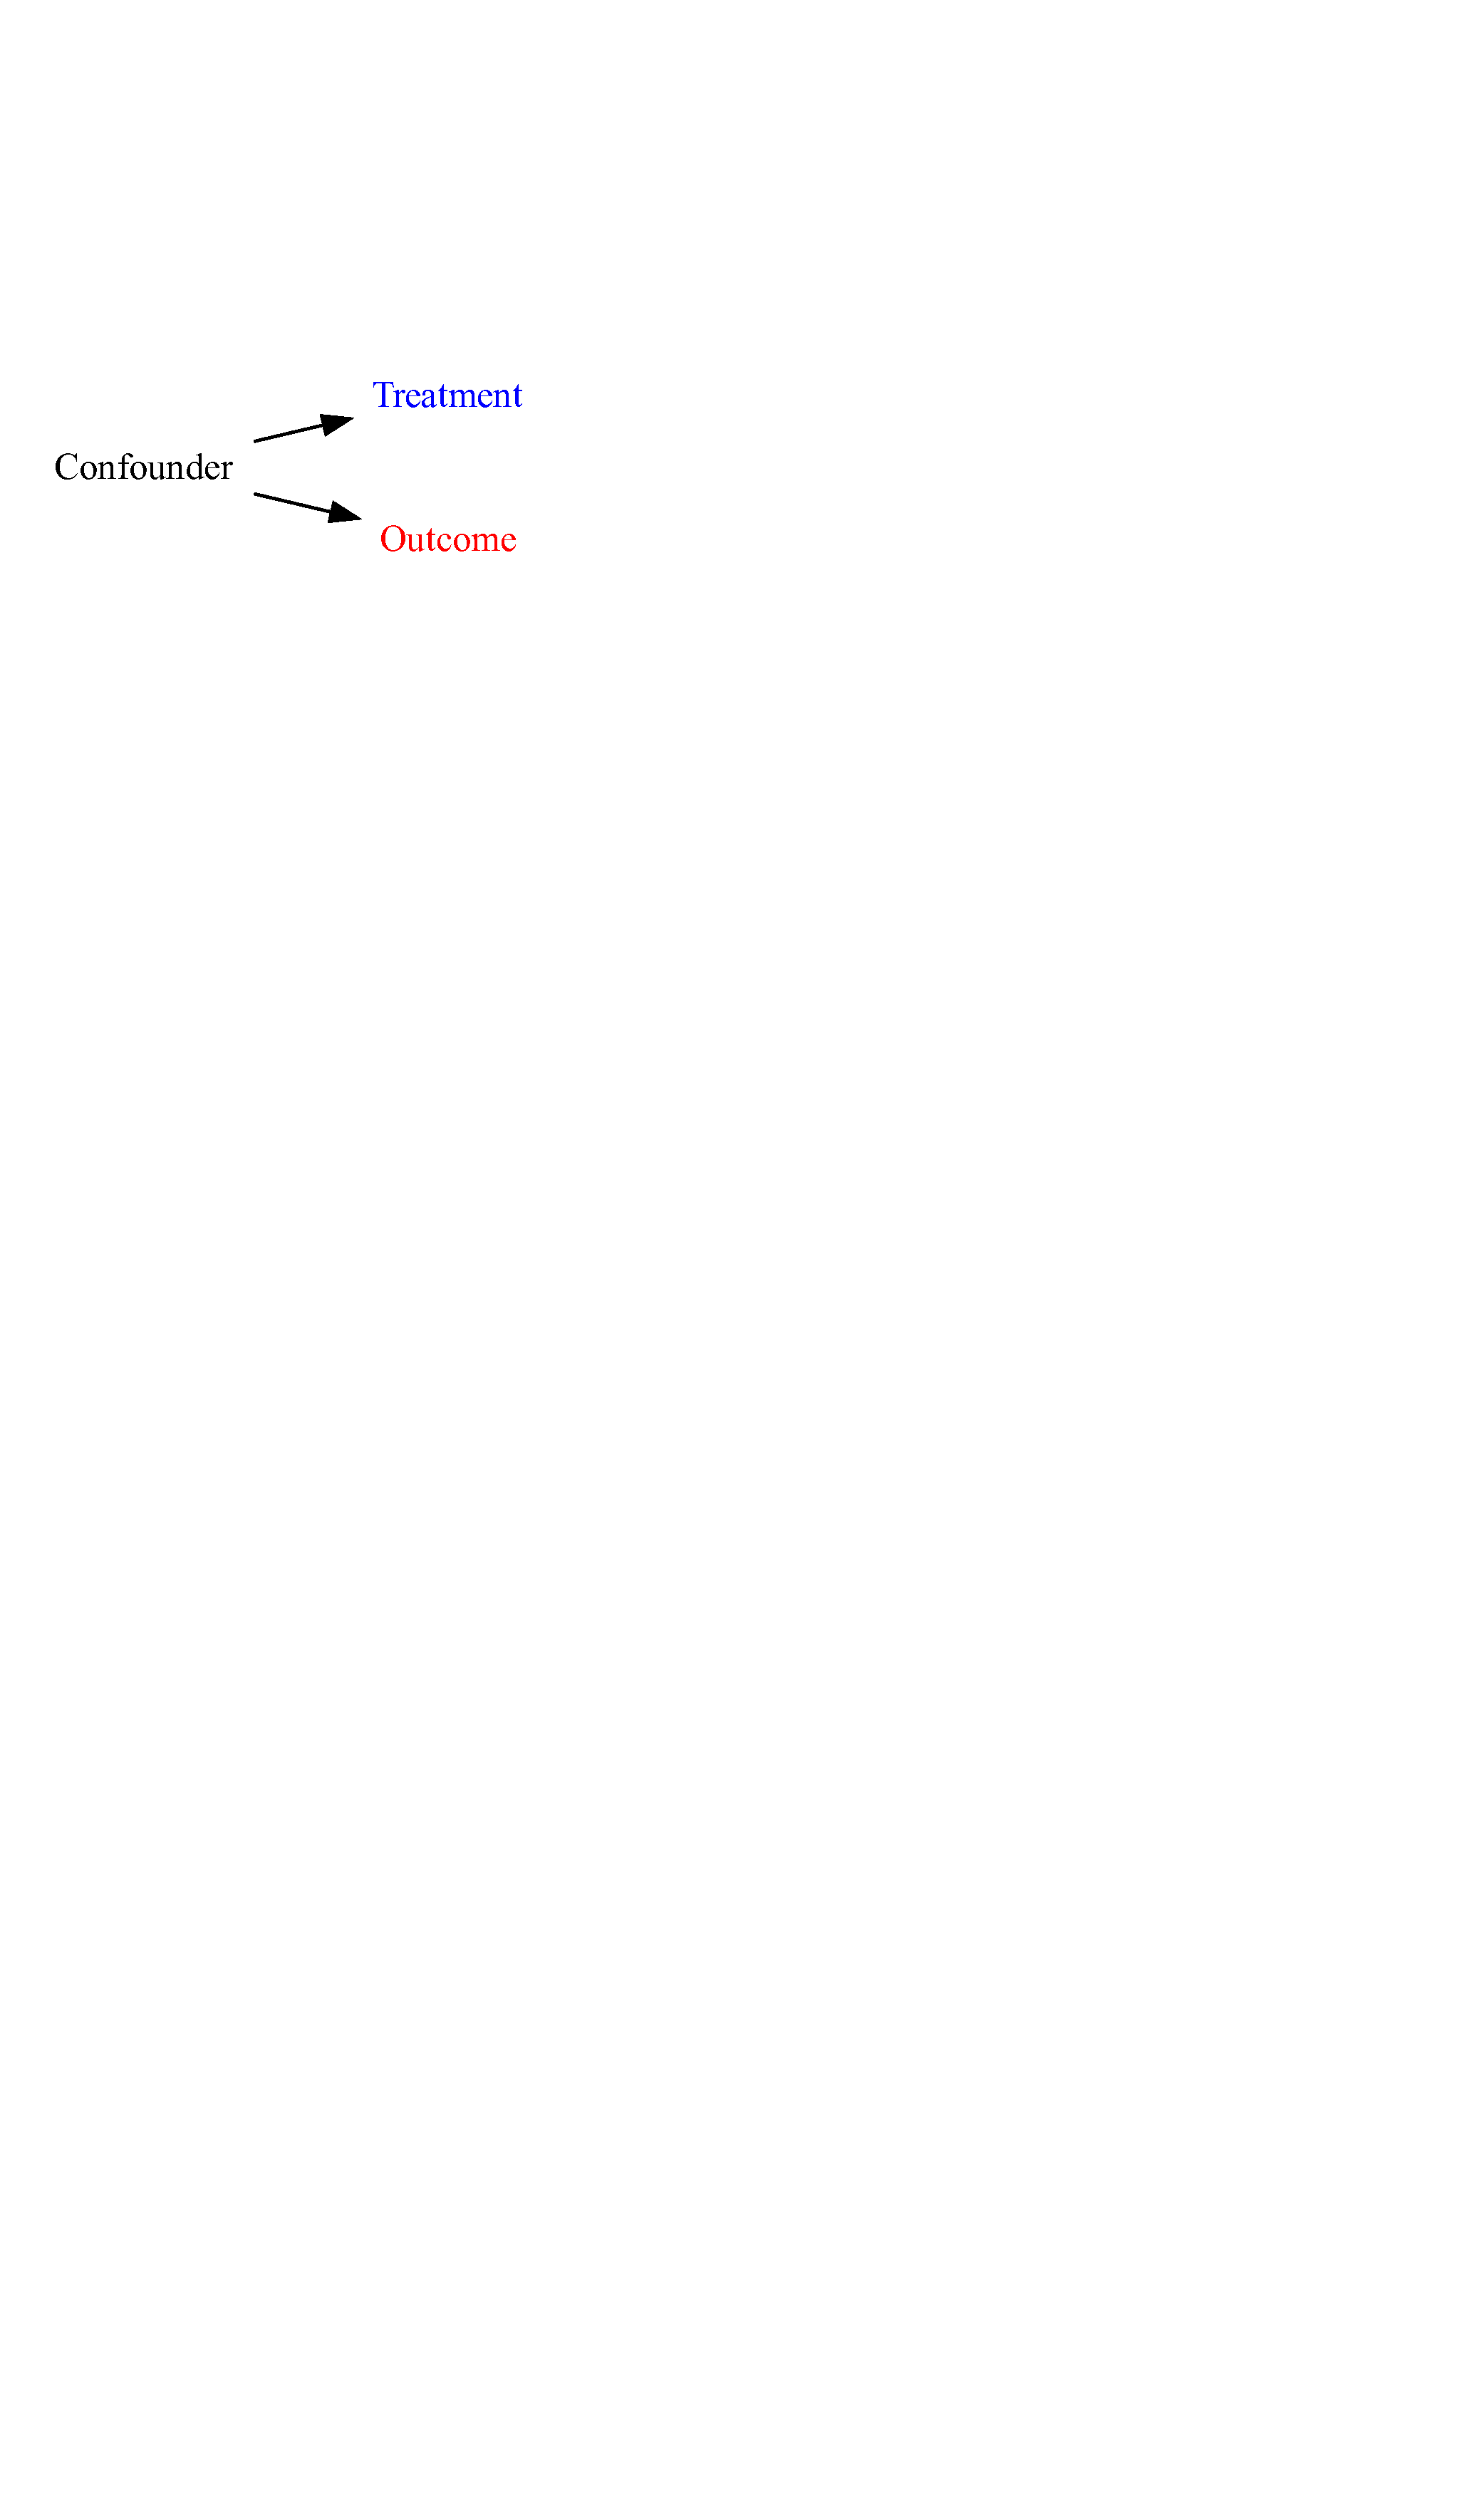
\includegraphics[width=1.4\linewidth]{figure/Dag2_a-1} 

\end{knitrout}
\end{frame}



\begin{frame}
\frametitle{Controlling for Confounding}
\begin{knitrout}
\definecolor{shadecolor}{rgb}{0.969, 0.969, 0.969}\color{fgcolor}
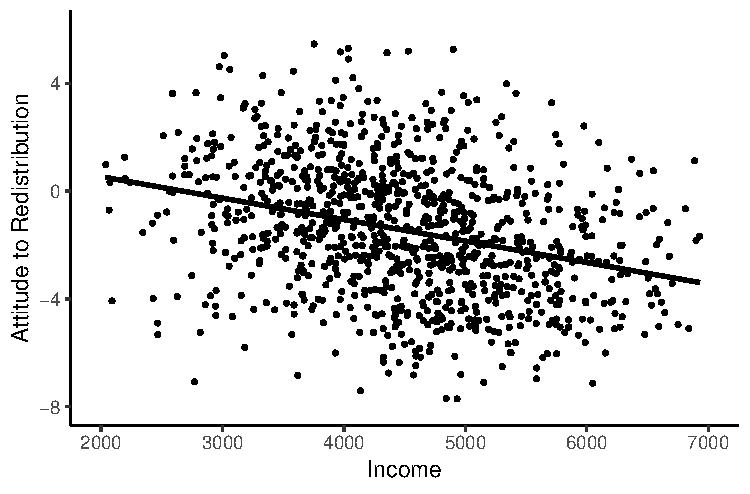
\includegraphics[width=\maxwidth]{figure/confound0a-1} 

\end{knitrout}
\end{frame}

\begin{frame}
\frametitle{Controlling for Confounding}
\begin{knitrout}
\definecolor{shadecolor}{rgb}{0.969, 0.969, 0.969}\color{fgcolor}
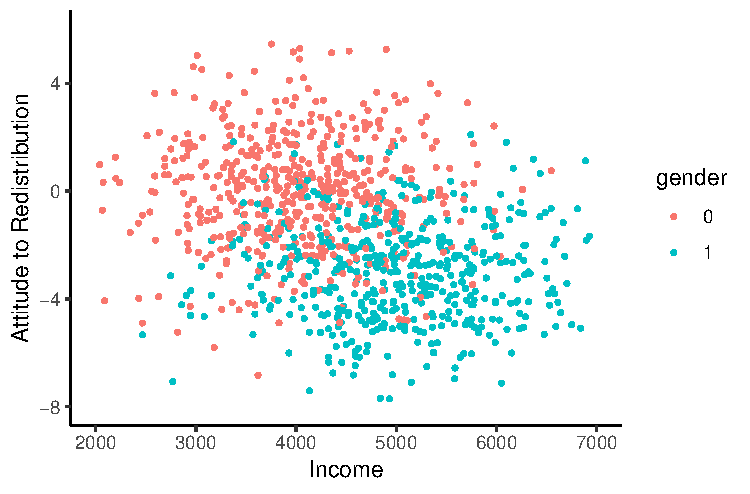
\includegraphics[width=\maxwidth]{figure/confound0b-1} 

\end{knitrout}
\end{frame}

\begin{frame}
\frametitle{Controlling for Confounding}
\begin{knitrout}
\definecolor{shadecolor}{rgb}{0.969, 0.969, 0.969}\color{fgcolor}
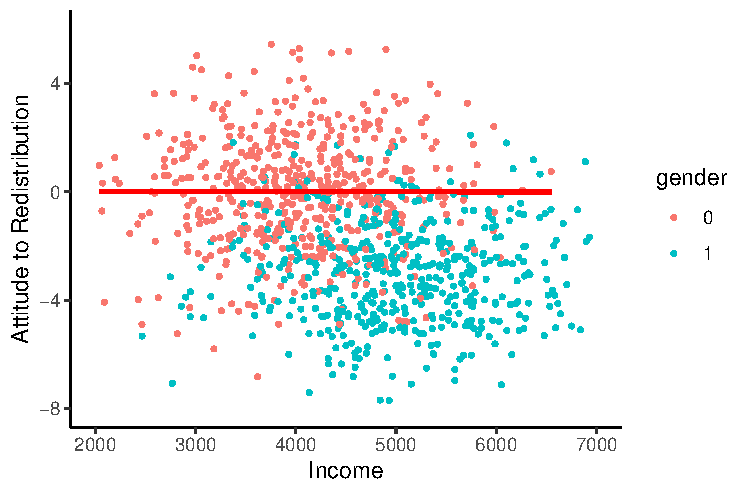
\includegraphics[width=\maxwidth]{figure/confound1a-1} 

\end{knitrout}
\end{frame}

\begin{frame}
\frametitle{Controlling for Confounding}
\begin{knitrout}
\definecolor{shadecolor}{rgb}{0.969, 0.969, 0.969}\color{fgcolor}
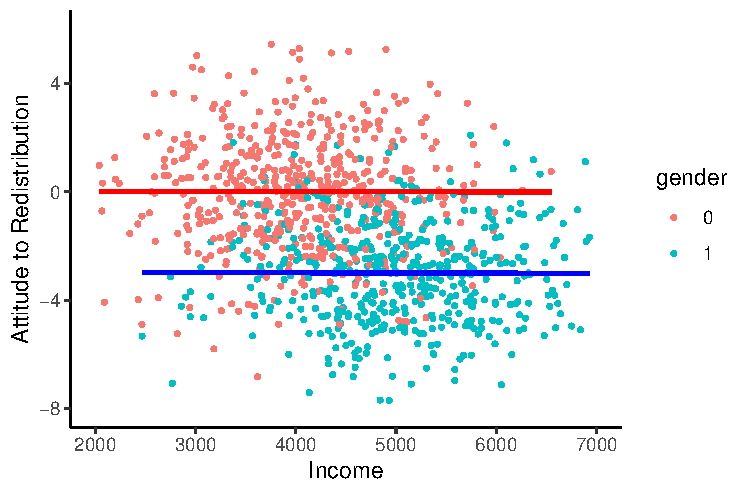
\includegraphics[width=\maxwidth]{figure/confound1b-1} 

\end{knitrout}
\end{frame}

\begin{frame}
\frametitle{Controlling for Confounding}
\begin{knitrout}
\definecolor{shadecolor}{rgb}{0.969, 0.969, 0.969}\color{fgcolor}
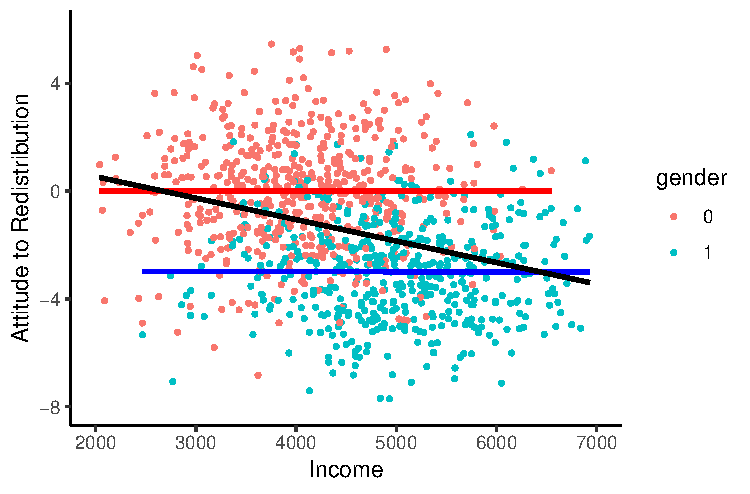
\includegraphics[width=\maxwidth]{figure/confound2-1} 

\end{knitrout}
\end{frame}

\begin{frame}
\frametitle{Controlling for Confounding}
\begin{itemize}
\footnotesize
\item If we omit a confounding variable, we bias our regression estimate:
\pause
\item 'True' regression with all confounders: 
\end{itemize}
$$ Y_i = \alpha + \beta D_i + \gamma X_i + \epsilon_i$$
\begin{itemize}
\pause
\footnotesize
\item The 'wrong' regression with a missing confounder:
\pause
\end{itemize}
$$ Y_i = \alpha + \beta D_i + \epsilon_i$$
\pause
\begin{itemize}
\footnotesize
\item What happens to our coefficient estimate?
\pause
\end{itemize}
$$ X_i = \psi + \delta D_i + \epsilon_i$$
\pause
$$ Y_i = \alpha + \beta D_i + \gamma (\psi + \delta D_i + \epsilon_i) + \epsilon_i $$
\pause
$$ Y_i = \alpha + D_i (\beta + \gamma \delta) + \gamma (\psi  + \epsilon_i) + \epsilon_i $$
\pause
\begin{itemize}
\footnotesize
\item So the coefficient we estimate is wrong by this amount:
\pause
$$ \beta_{wrong} = \beta_{true} + \gamma \delta$$
\end{itemize}
\normalsize
\end{frame}


\begin{frame}
\frametitle{Controlling for Confounding}
\begin{itemize}
\item What does controlling \textbf{do}?
\begin{itemize}
\pause 
\item It means \textbf{removing the variation} in the data due to the confounder
\pause
\item Equivalently, it means separating our data for each value of the confounder: \textbf{Subclassification}
\pause
\item Then, within each group, the confounder is \textbf{constant} and can't affect the relationship between $D$ and $Y$.
\pause
\item We have \textbf{created balance} between the treated and control groups on the confounder
\end{itemize}
\end{itemize}
\end{frame}

\begin{frame}
\frametitle{Controlling for Confounding}
\begin{itemize}
\item We receive a dataset with twenty variables: $D$, $Y$ and 18 more. 
\begin{itemize}
\item Which variables should we include as controls?
\end{itemize}
\pause
\item We usually should \textbf{NOT} include all of them
\pause
\begin{itemize}
\item Only the variables \textbf{necessary} to stop confounding
\pause
\item Including unnecessary variables can produce bias
\begin{itemize}
\item "Bad controls"/"Post-treatment Bias"
\end{itemize}
\pause
\item We lose power (degrees of freedom) for every control we add
\pause
\item And additional variables reduce overlap (increase model-dependence)
\pause
\end{itemize}
\end{itemize}
\end{frame}

\section{Which Variables to Control For}

\begin{frame}
\frametitle{Causal Diagrams (DAGs)}
\begin{itemize}
\item To know which variables to control for, it helps to draw a causal diagram
\pause
\begin{itemize}
\item A \textbf{Directed Acyclical Graph} (DAG)
\pause
\item Arrows only in one direction
\pause
\item No circular loops!
\end{itemize}
\end{itemize}
\end{frame}

\begin{frame}
\frametitle{Causal Diagrams (DAGs)}
\begin{knitrout}
\definecolor{shadecolor}{rgb}{0.969, 0.969, 0.969}\color{fgcolor}
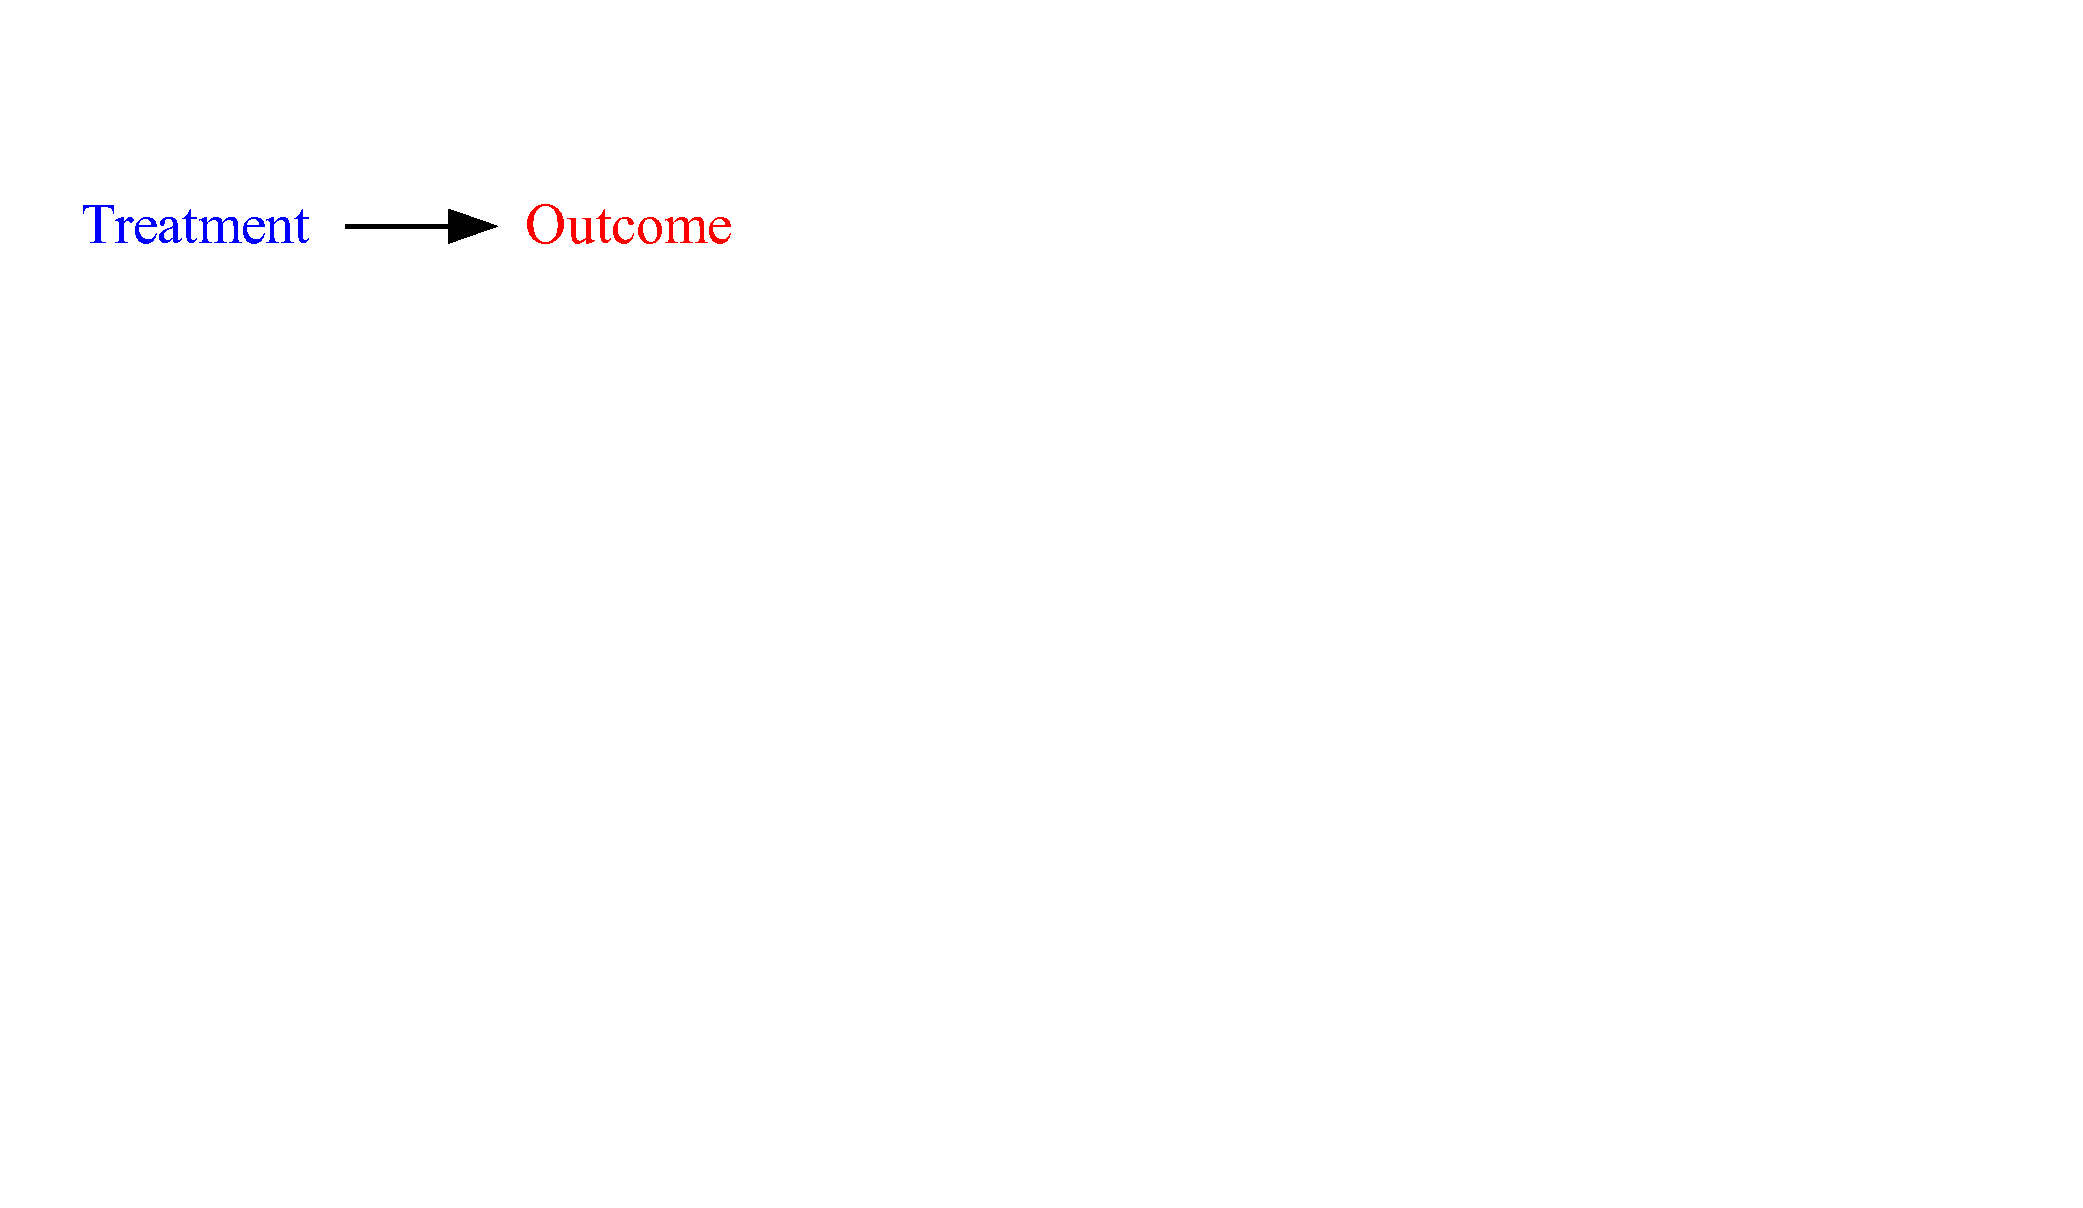
\includegraphics[width=1.8\linewidth]{figure/Dag1-1} 

\end{knitrout}
\end{frame}

\begin{frame}
\frametitle{Causal Diagrams (DAGs)}
\begin{itemize}
\item Causation is like \textbf{Water}, flowing along the graph
\begin{itemize}
\item We want to focus on one 'flow' of causation from treatment to outcomes
\pause
\item Avoiding mixing with the other flows of causation in the network
\end{itemize}
\end{itemize}
\end{frame}

\begin{frame}
\frametitle{Causal Diagrams (DAGs)}
\begin{knitrout}
\definecolor{shadecolor}{rgb}{0.969, 0.969, 0.969}\color{fgcolor}
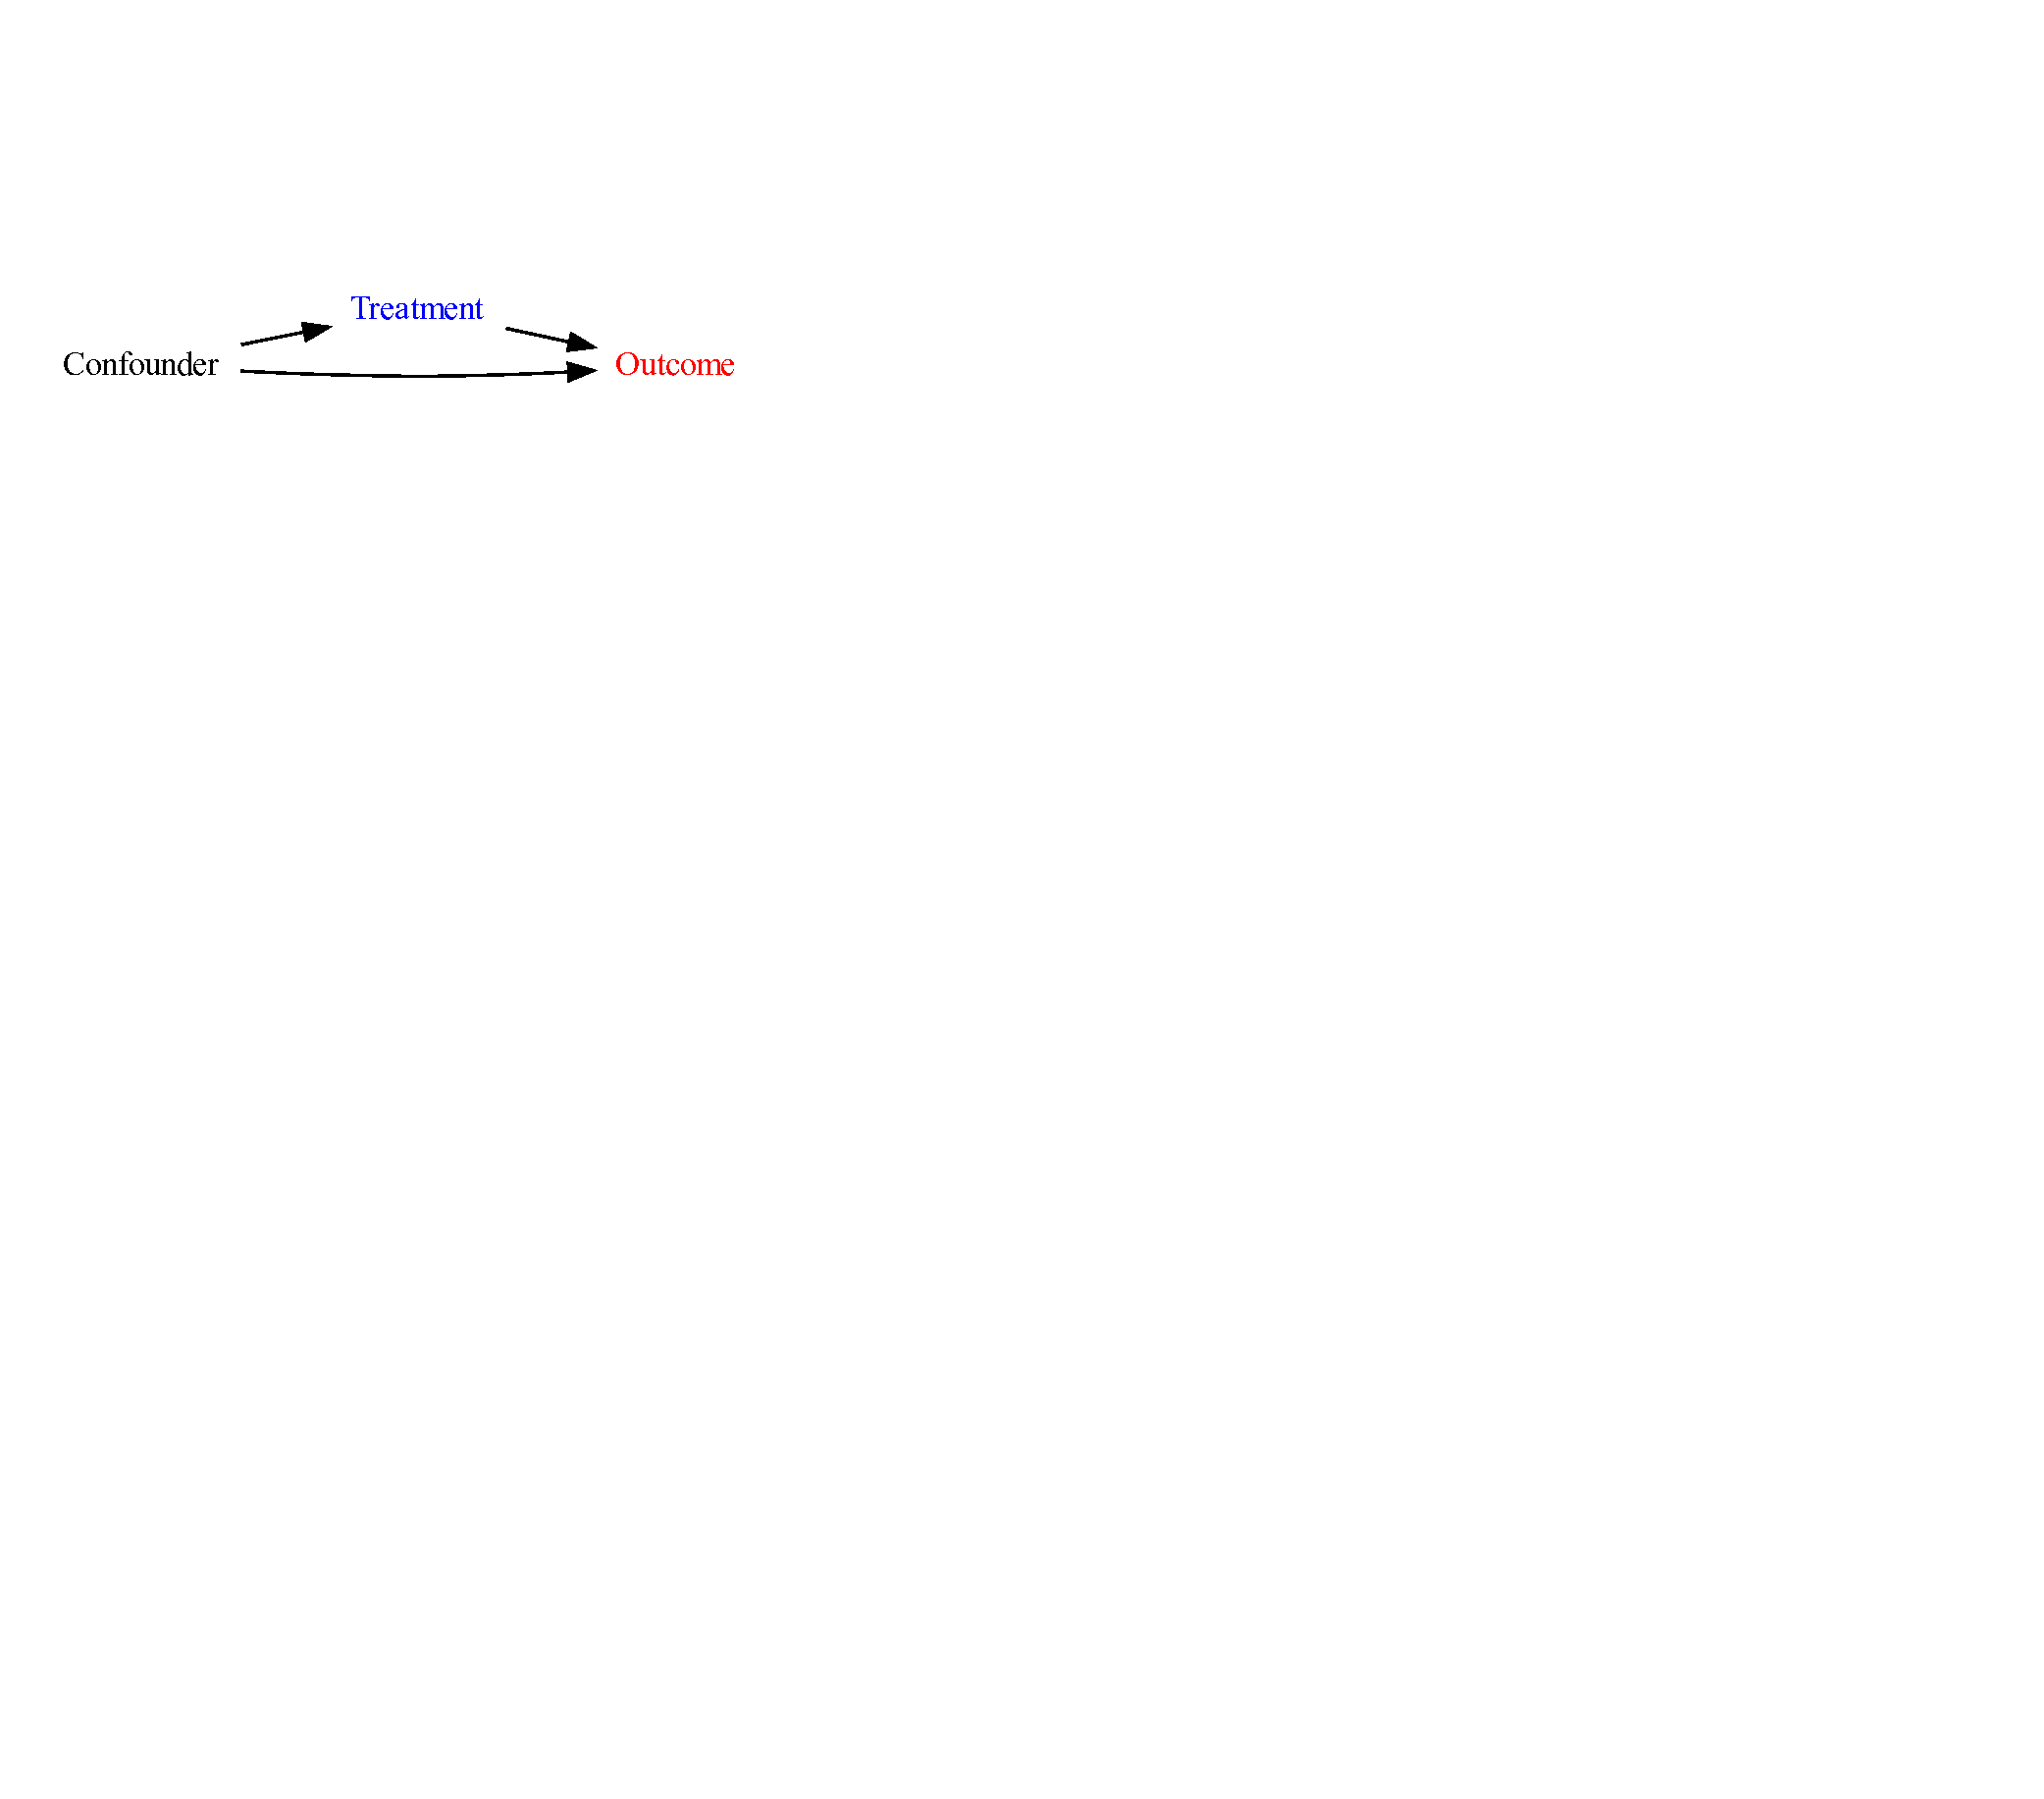
\includegraphics[width=1.8\linewidth]{figure/Dag2-1} 

\end{knitrout}
\end{frame}

\begin{frame}
\frametitle{Causal Diagrams (DAGs)}
\begin{itemize}
\item Three Rules to achieve Conditional Independence:
\begin{enumerate}
\item Include as controls enough variables to \textbf{block all back-door paths} from treatment to the outcome
\pause
\item Exclude any variables that are \textbf{post-treatment}
\pause
\item Exclude any variables that are \textbf{colliders}
\end{enumerate}
\end{itemize}
\end{frame}

\begin{frame}
\frametitle{1. Back-door Paths}
\begin{itemize}
\item To identify back-door paths:
\pause
\begin{itemize}
\item Start with an arrow pointing at treatment
\pause
\item Trace the path 'backwards' (the direction of the arrows doesn't matter) until you reach the outcome
\pause
\item Repeat for every possible path from treatment to outcome
\pause
\end{itemize}
\item \textbf{Block back-door paths} by controlling for any variable along the path
\pause
\item Identify the \textbf{Minimum set of controls} that blocks \textit{All} back-door paths
\pause
\begin{itemize}
\item This achieves conditional independence of treatment from potential outcomes!
\pause
\item Include these as control variables in our regression
\end{itemize}
\end{itemize}
\end{frame}

\begin{frame}
\frametitle{1. Back-door Paths}
\begin{knitrout}
\definecolor{shadecolor}{rgb}{0.969, 0.969, 0.969}\color{fgcolor}
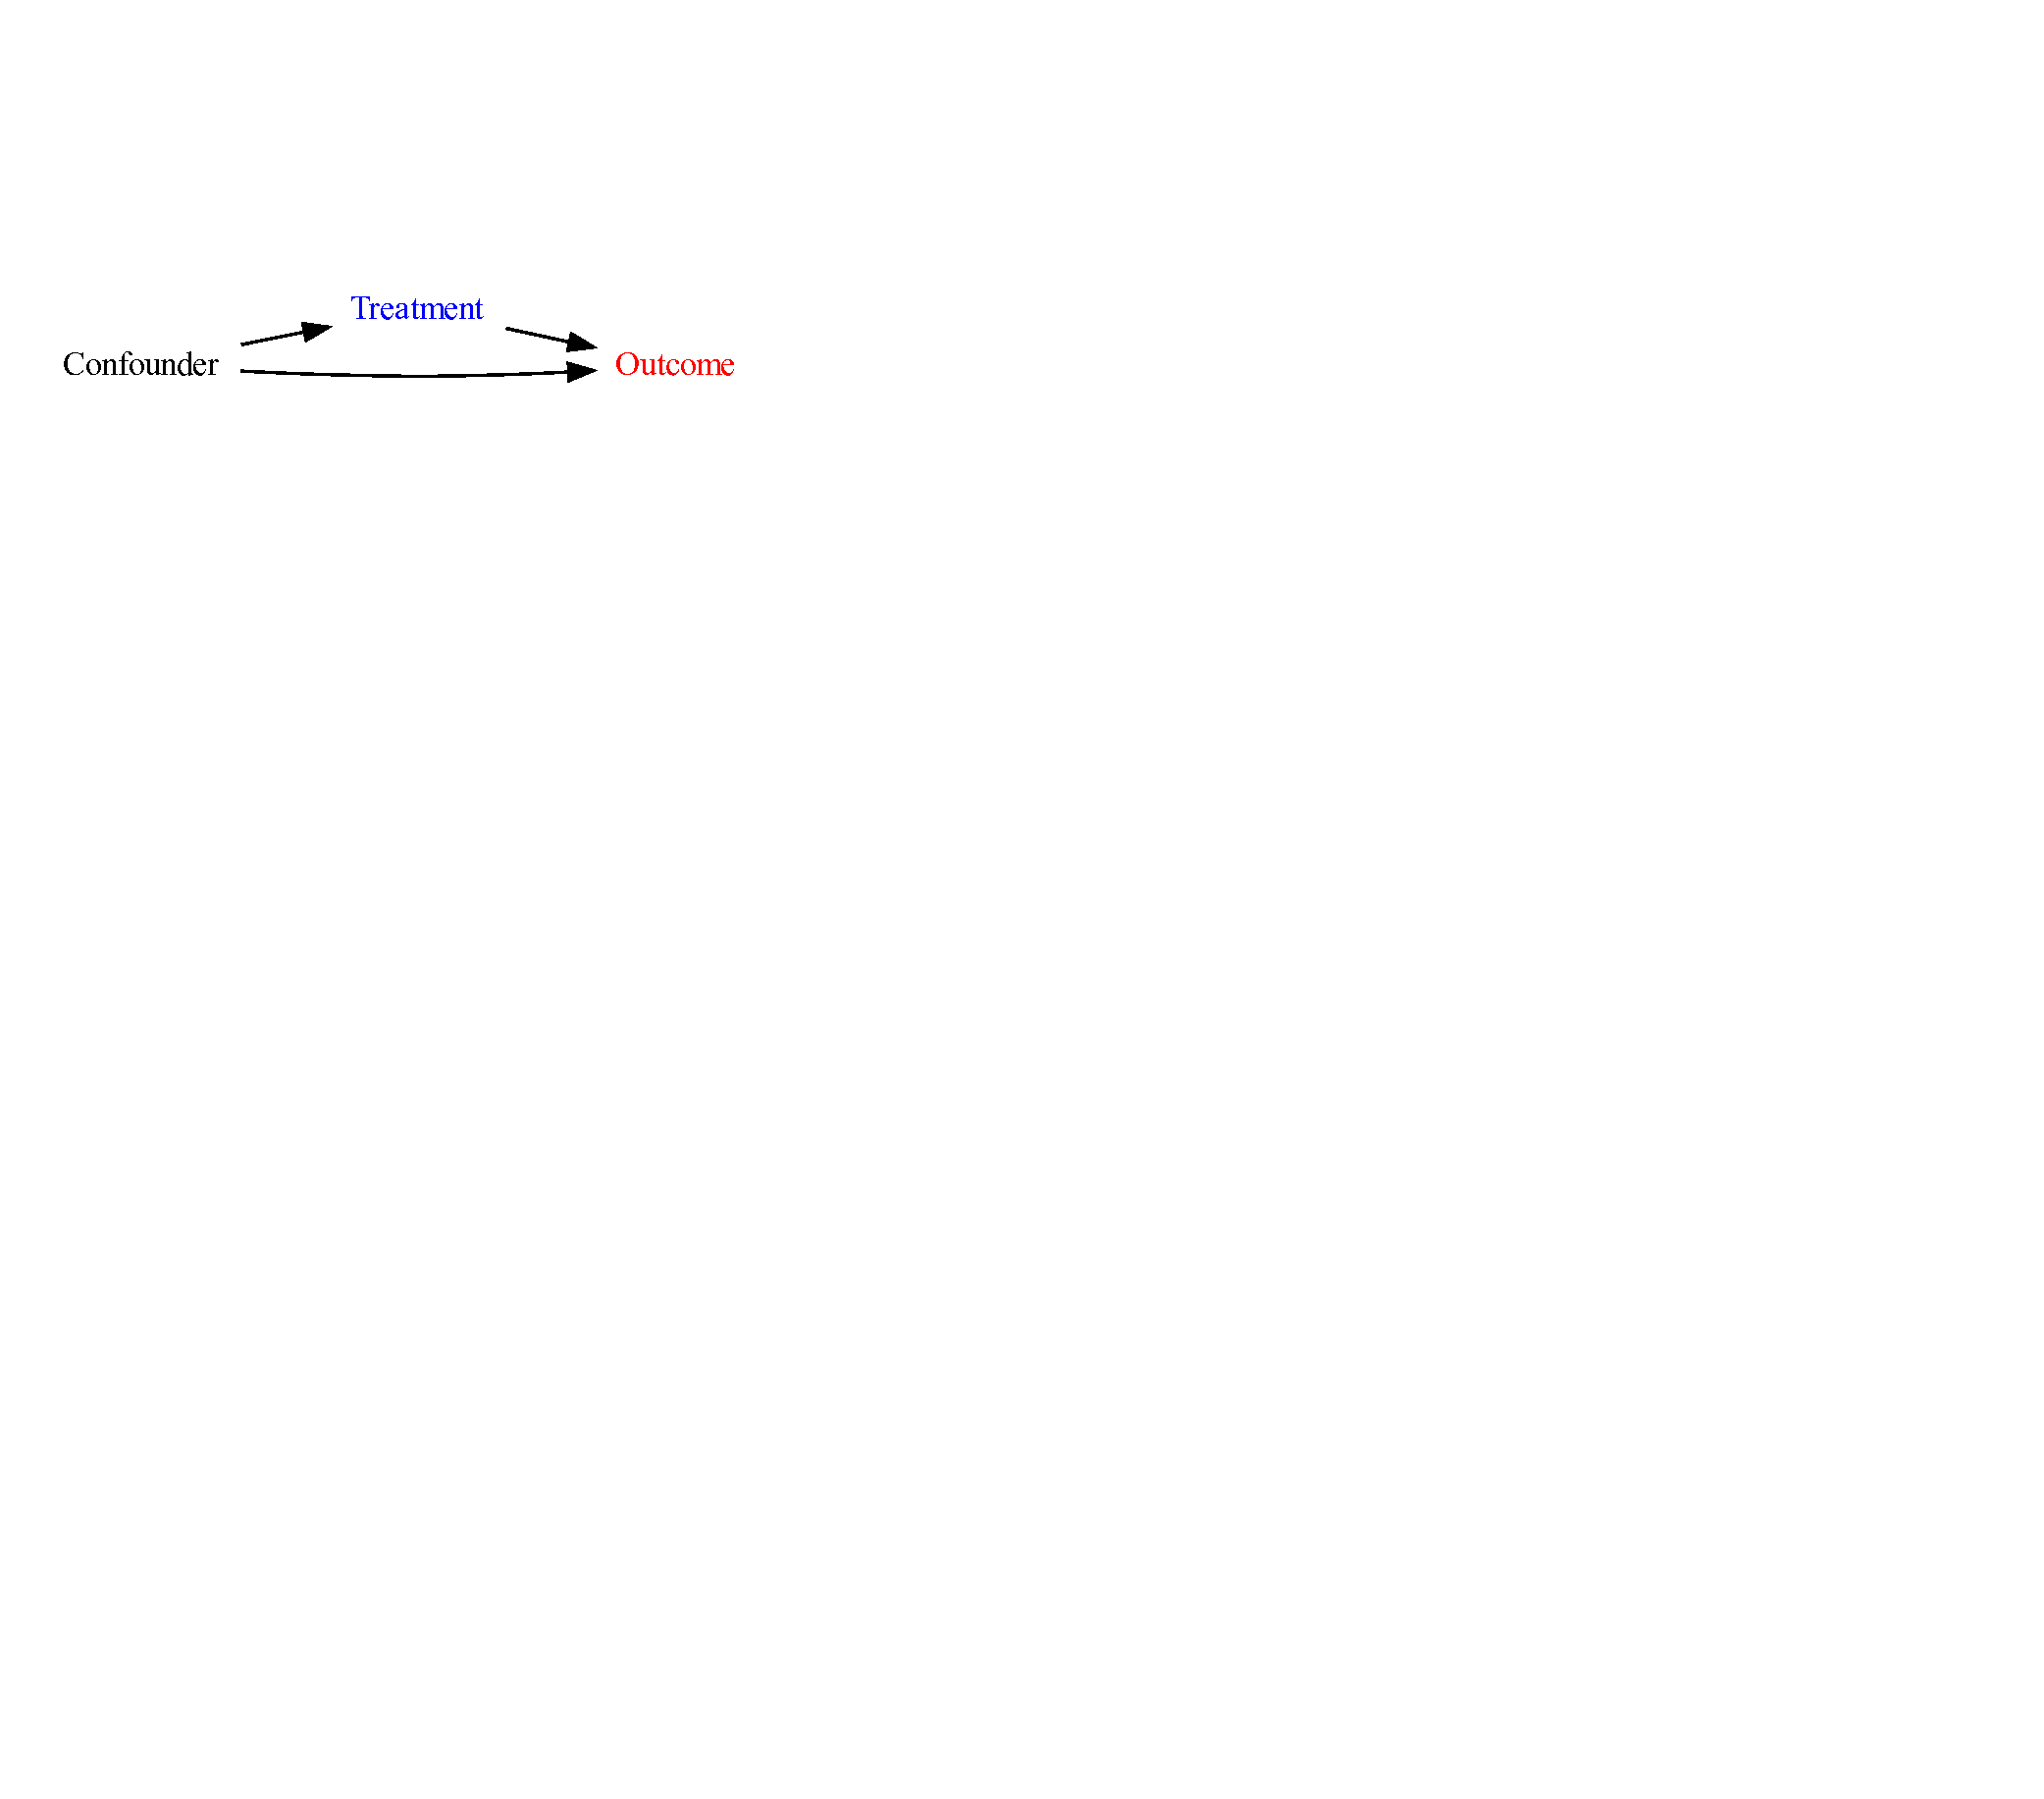
\includegraphics[width=2.5\linewidth]{figure/Dag2b-1} 

\end{knitrout}
\end{frame}

\begin{frame}
\frametitle{1. Back-door Paths}
\begin{knitrout}
\definecolor{shadecolor}{rgb}{0.969, 0.969, 0.969}\color{fgcolor}
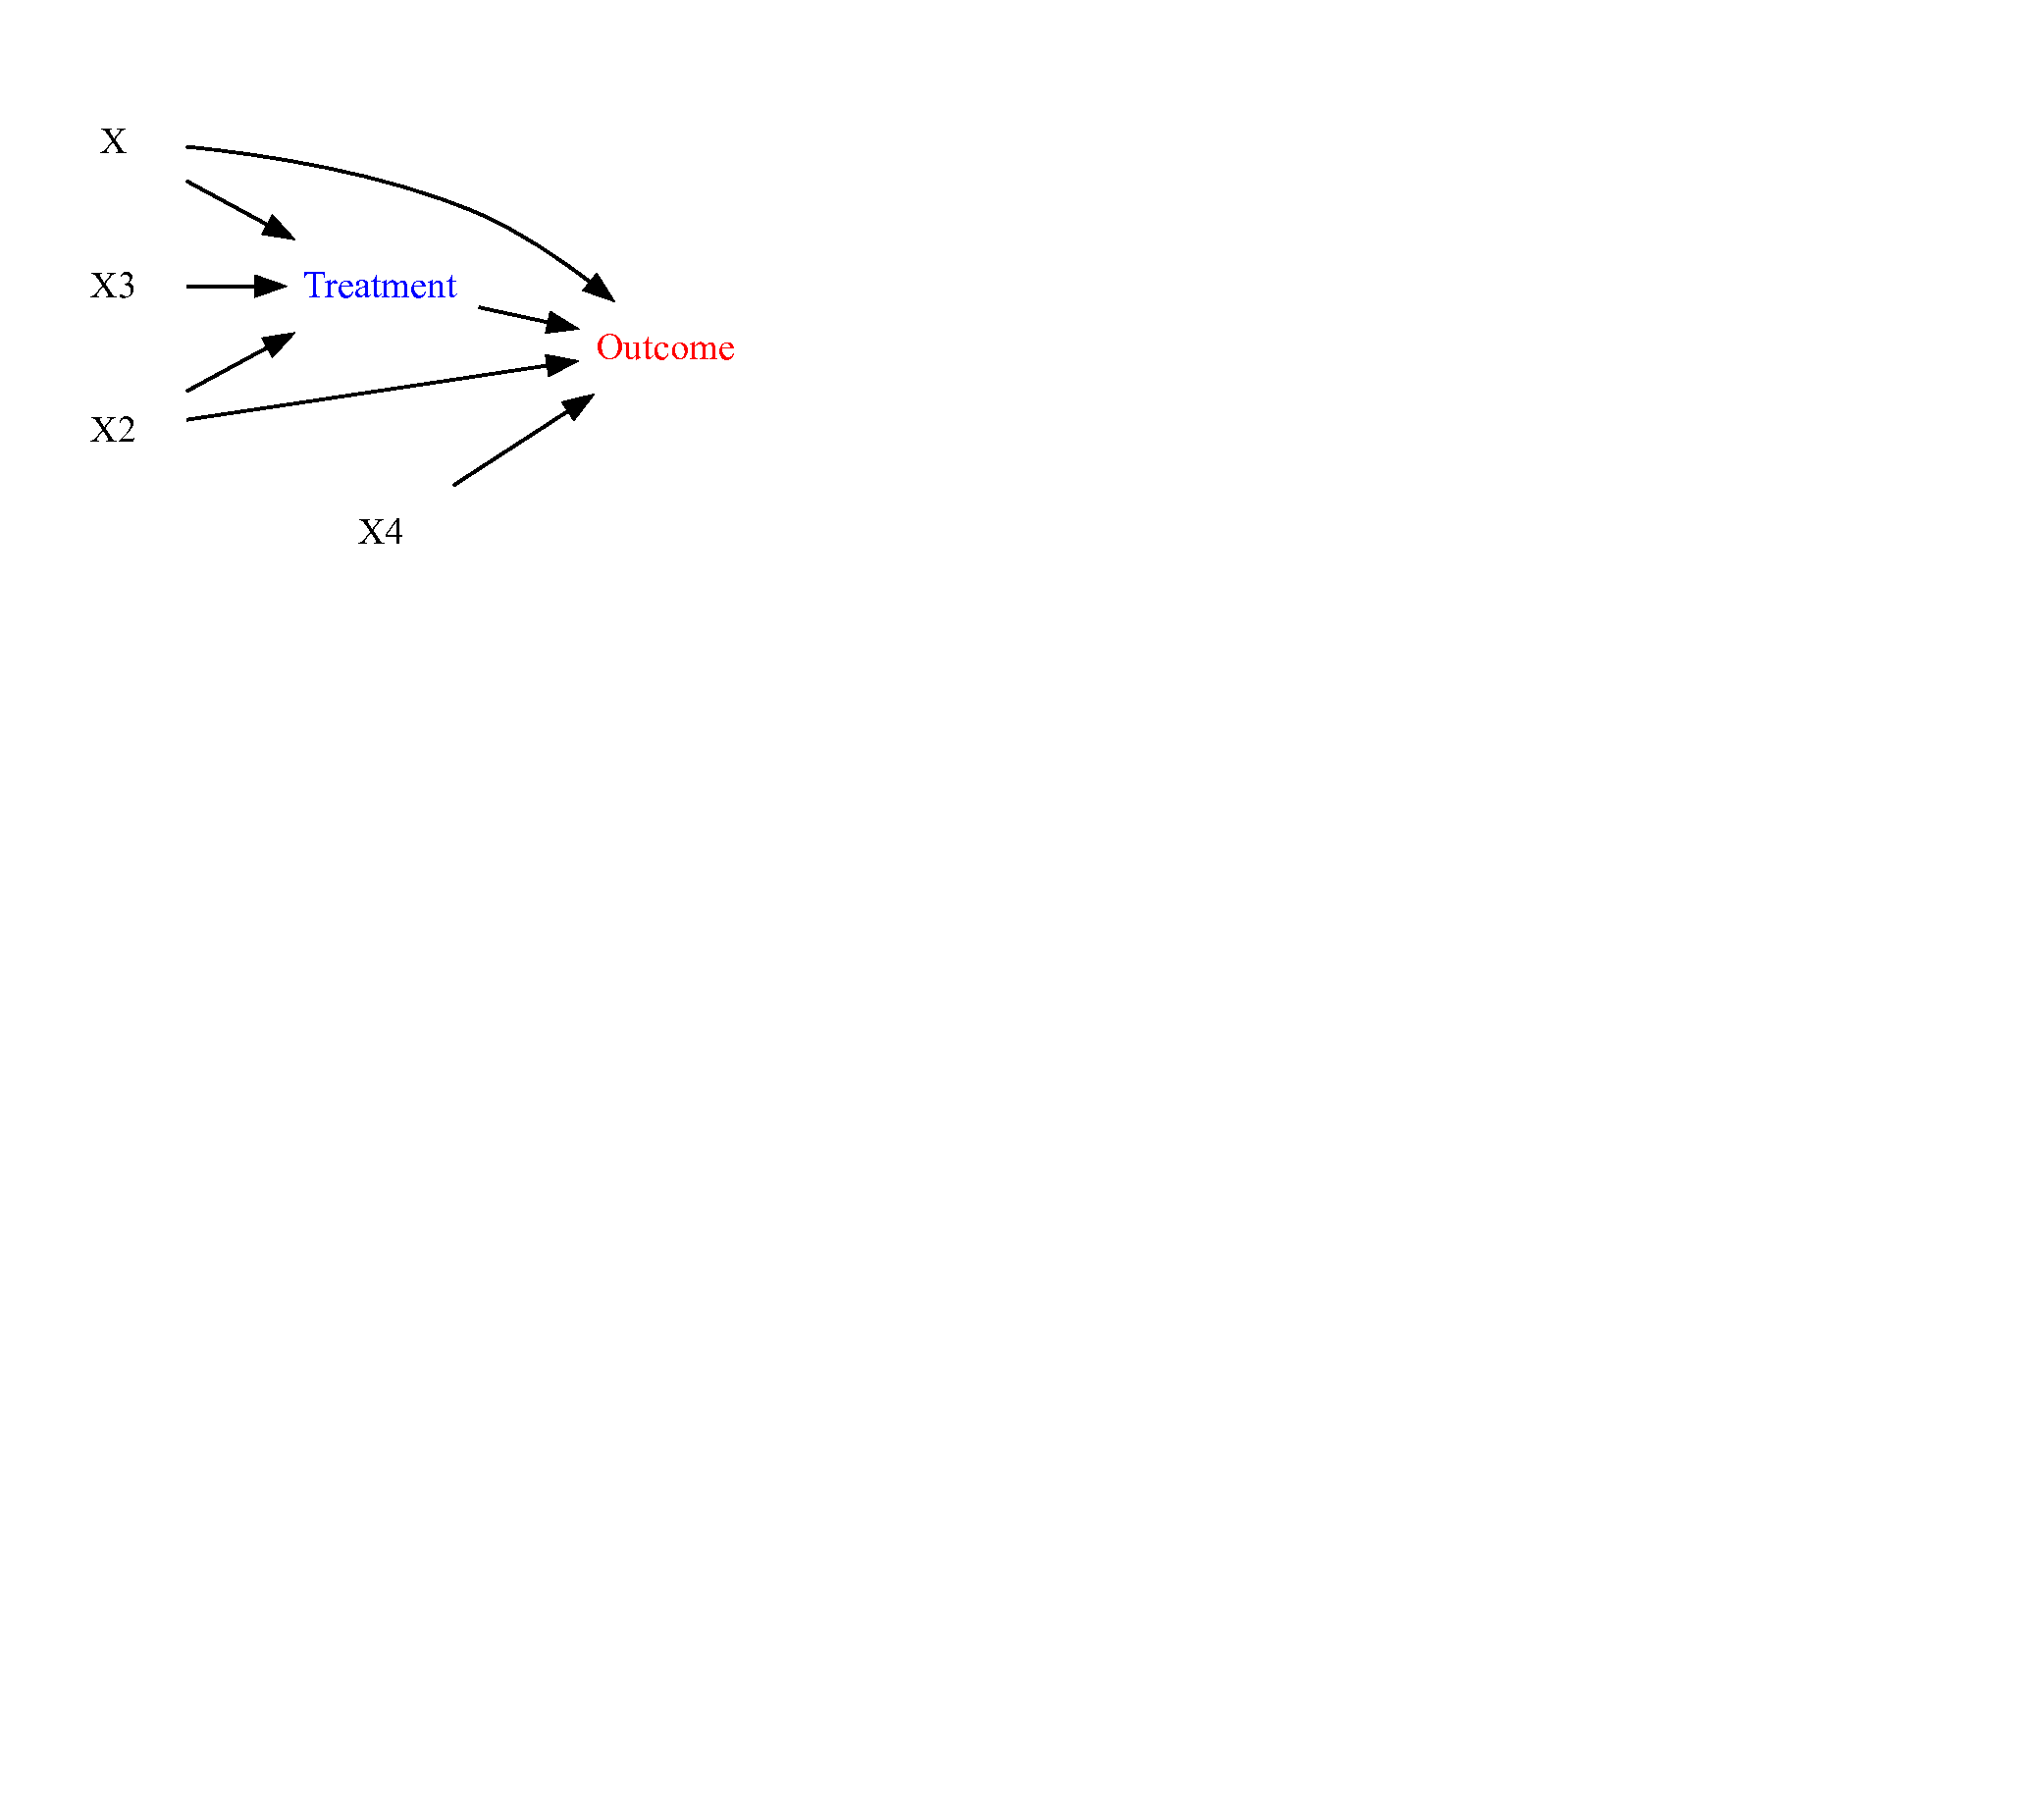
\includegraphics[width=2.5\linewidth]{figure/Dag2c-1} 

\end{knitrout}
\end{frame}

\begin{frame}
\frametitle{1. Back-door Paths}
\begin{knitrout}
\definecolor{shadecolor}{rgb}{0.969, 0.969, 0.969}\color{fgcolor}
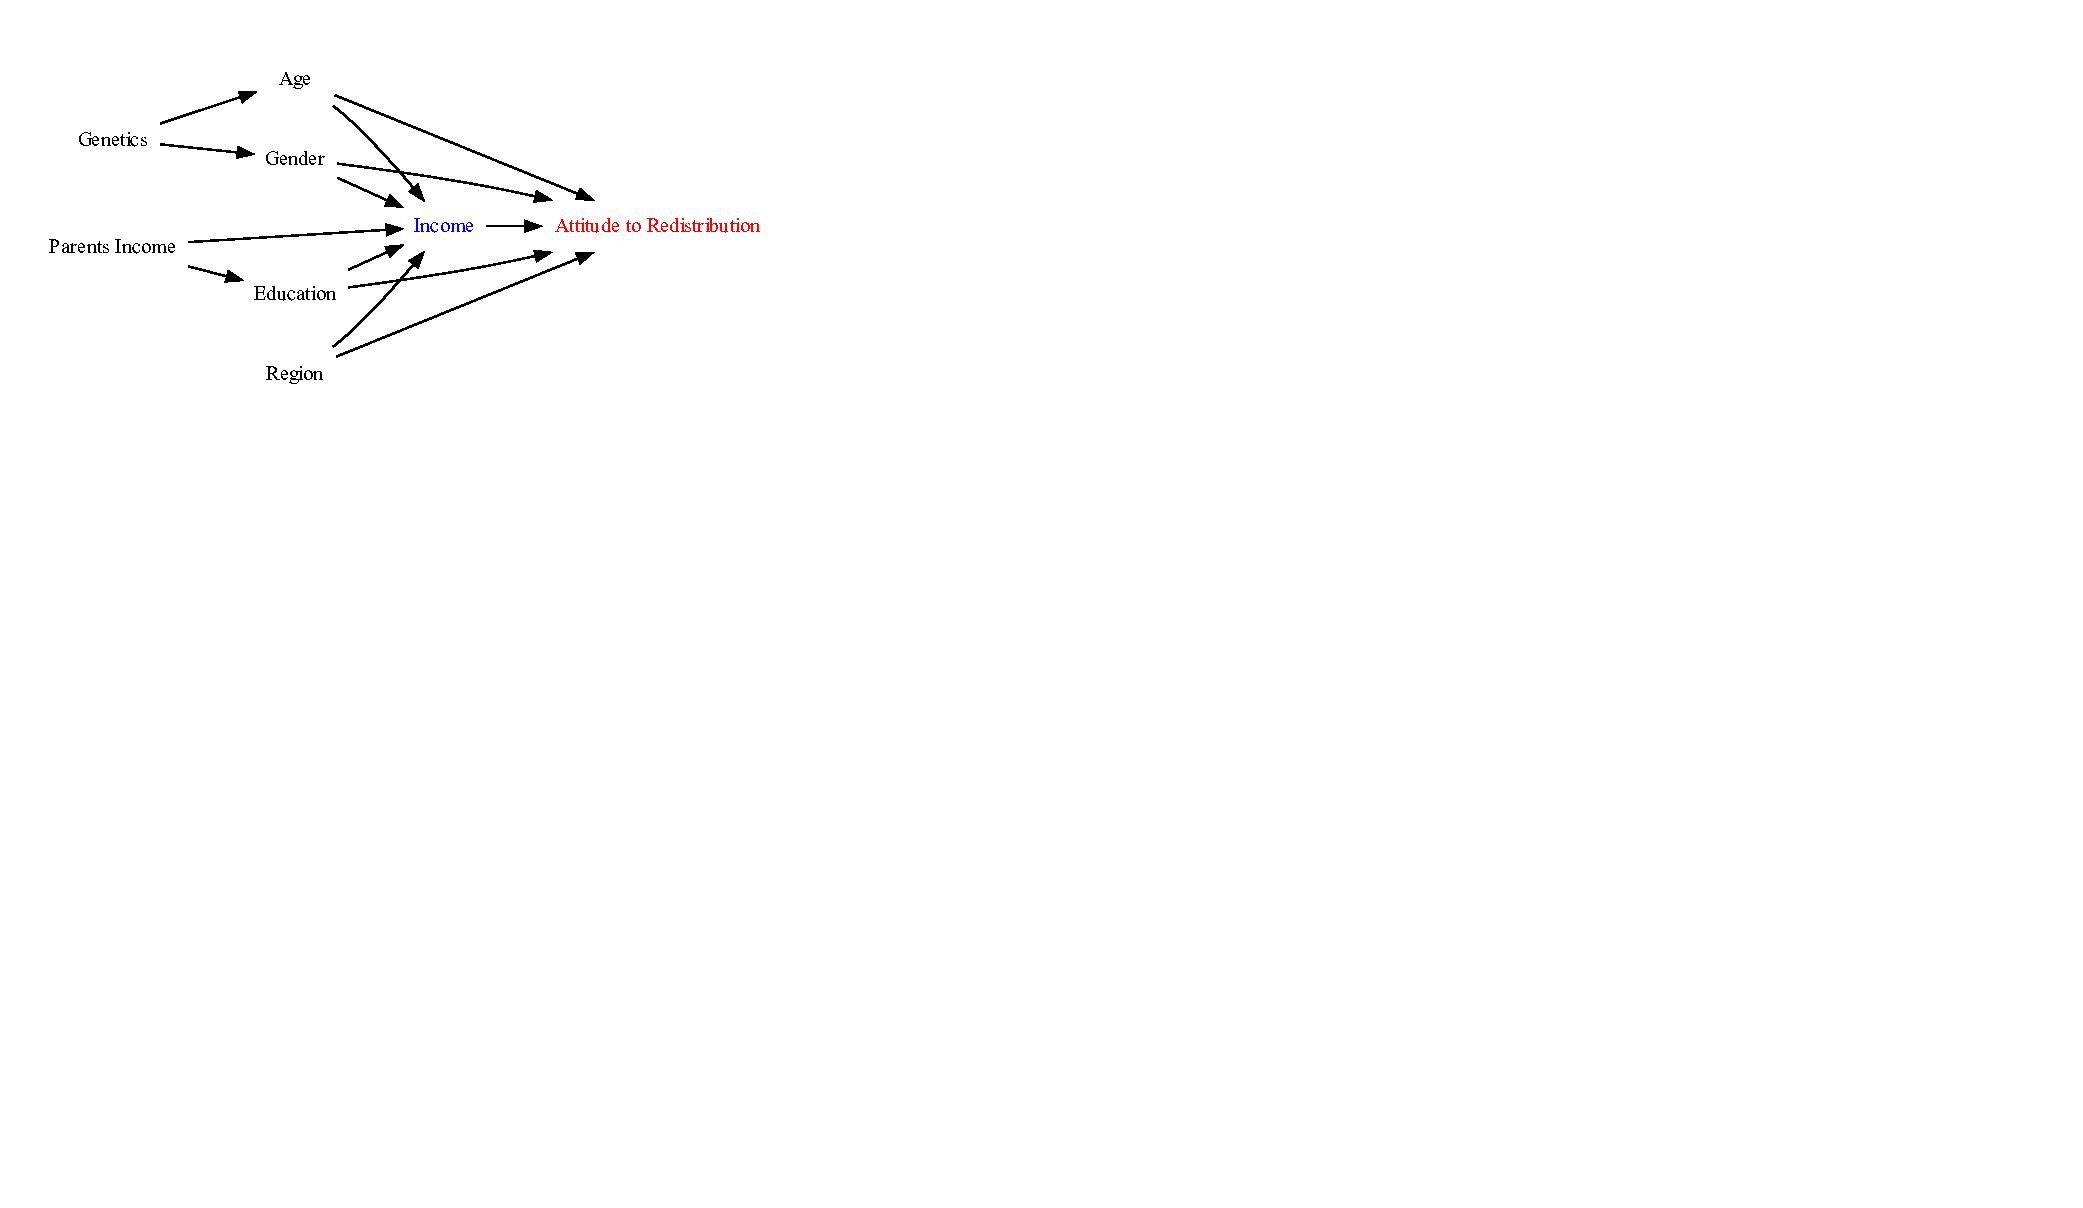
\includegraphics[width=2.7\linewidth]{figure/Dag4_paths_b-1} 

\end{knitrout}
\end{frame}

\begin{frame}
\frametitle{1. Back-door Paths}
\begin{knitrout}
\definecolor{shadecolor}{rgb}{0.969, 0.969, 0.969}\color{fgcolor}
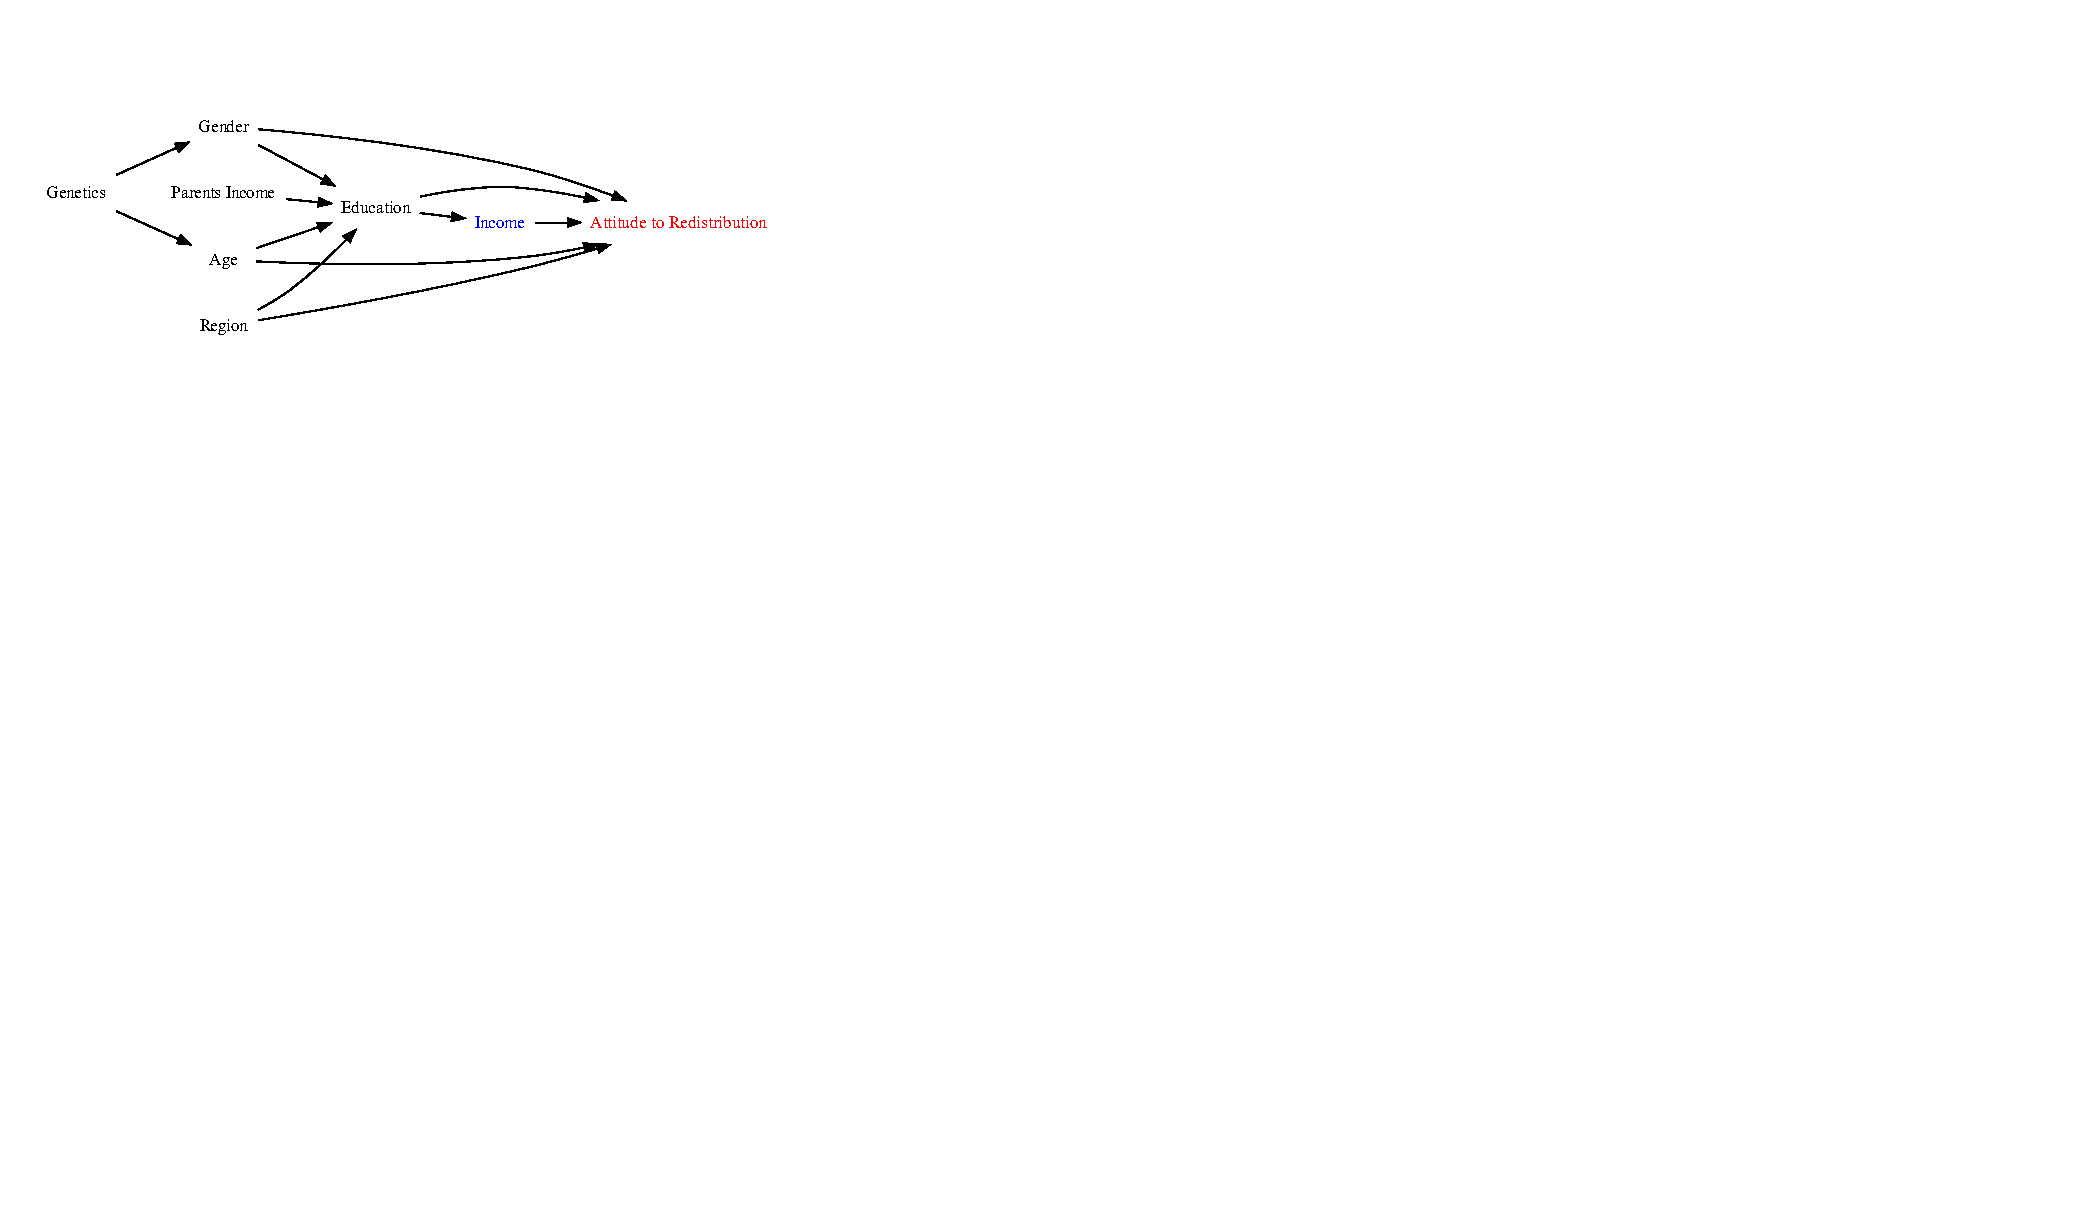
\includegraphics[width=2.7\linewidth]{figure/Dag4_paths_c-1} 

\end{knitrout}
\end{frame}

\begin{frame}
\frametitle{2. Post-treatment Variables}
\begin{itemize}
\item Including \textbf{post-treatment} variables will introduce bias
\pause
\begin{itemize}
\item Because variables measured 'after' treatment can also be affected by treatment
\pause
\item They're not confounders, but mechanisms/\textbf{mediating variables}
\pause
\item Controlling for them changes the definition of the causal effect we are estimating
\end{itemize}
\end{itemize}
\end{frame}

\begin{frame}
\frametitle{2. Post-treatment Variables}
\begin{knitrout}
\definecolor{shadecolor}{rgb}{0.969, 0.969, 0.969}\color{fgcolor}
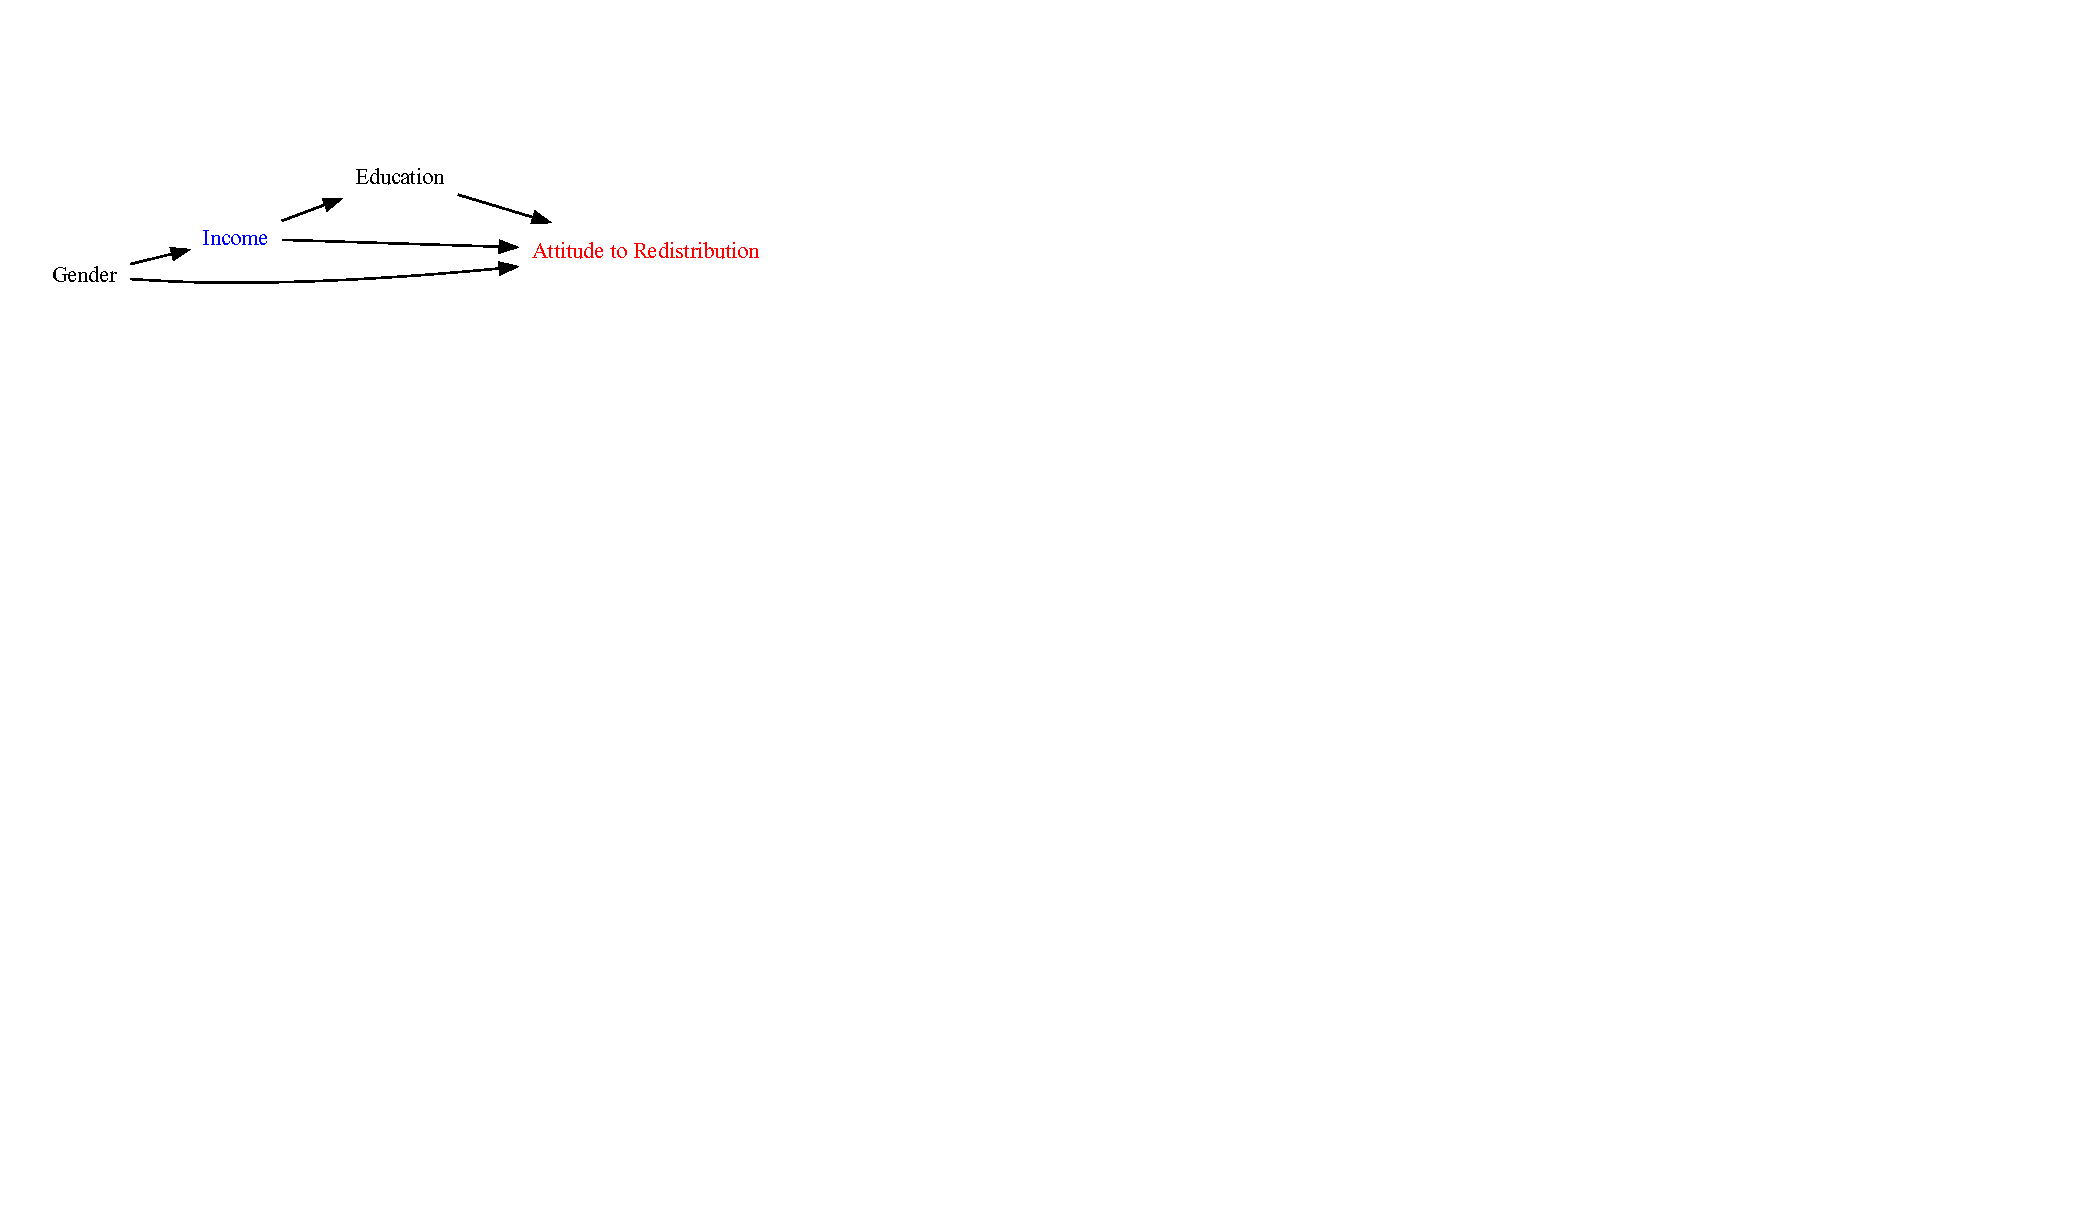
\includegraphics[width=2.7\linewidth]{figure/Dag4-1} 

\end{knitrout}
\end{frame}

\begin{frame}
\frametitle{3. Colliders}
\begin{itemize}
\item Colliders are variables on back-door paths which have arrows pointing both into them \textit{and} out of them
\pause
\item The water 'collides' in both directions so the source variables are not correlated, and produce no bias
\pause
\item But if we do accidentally 'control' for a collider we \textit{introduce} a bias in the relationship between $D$ and $Y$
\pause
\item So we must avoid controlling for colliders
\pause
\item Hard!
\end{itemize}
\end{frame}

\begin{frame}
\frametitle{3. Colliders}
\begin{knitrout}
\definecolor{shadecolor}{rgb}{0.969, 0.969, 0.969}\color{fgcolor}
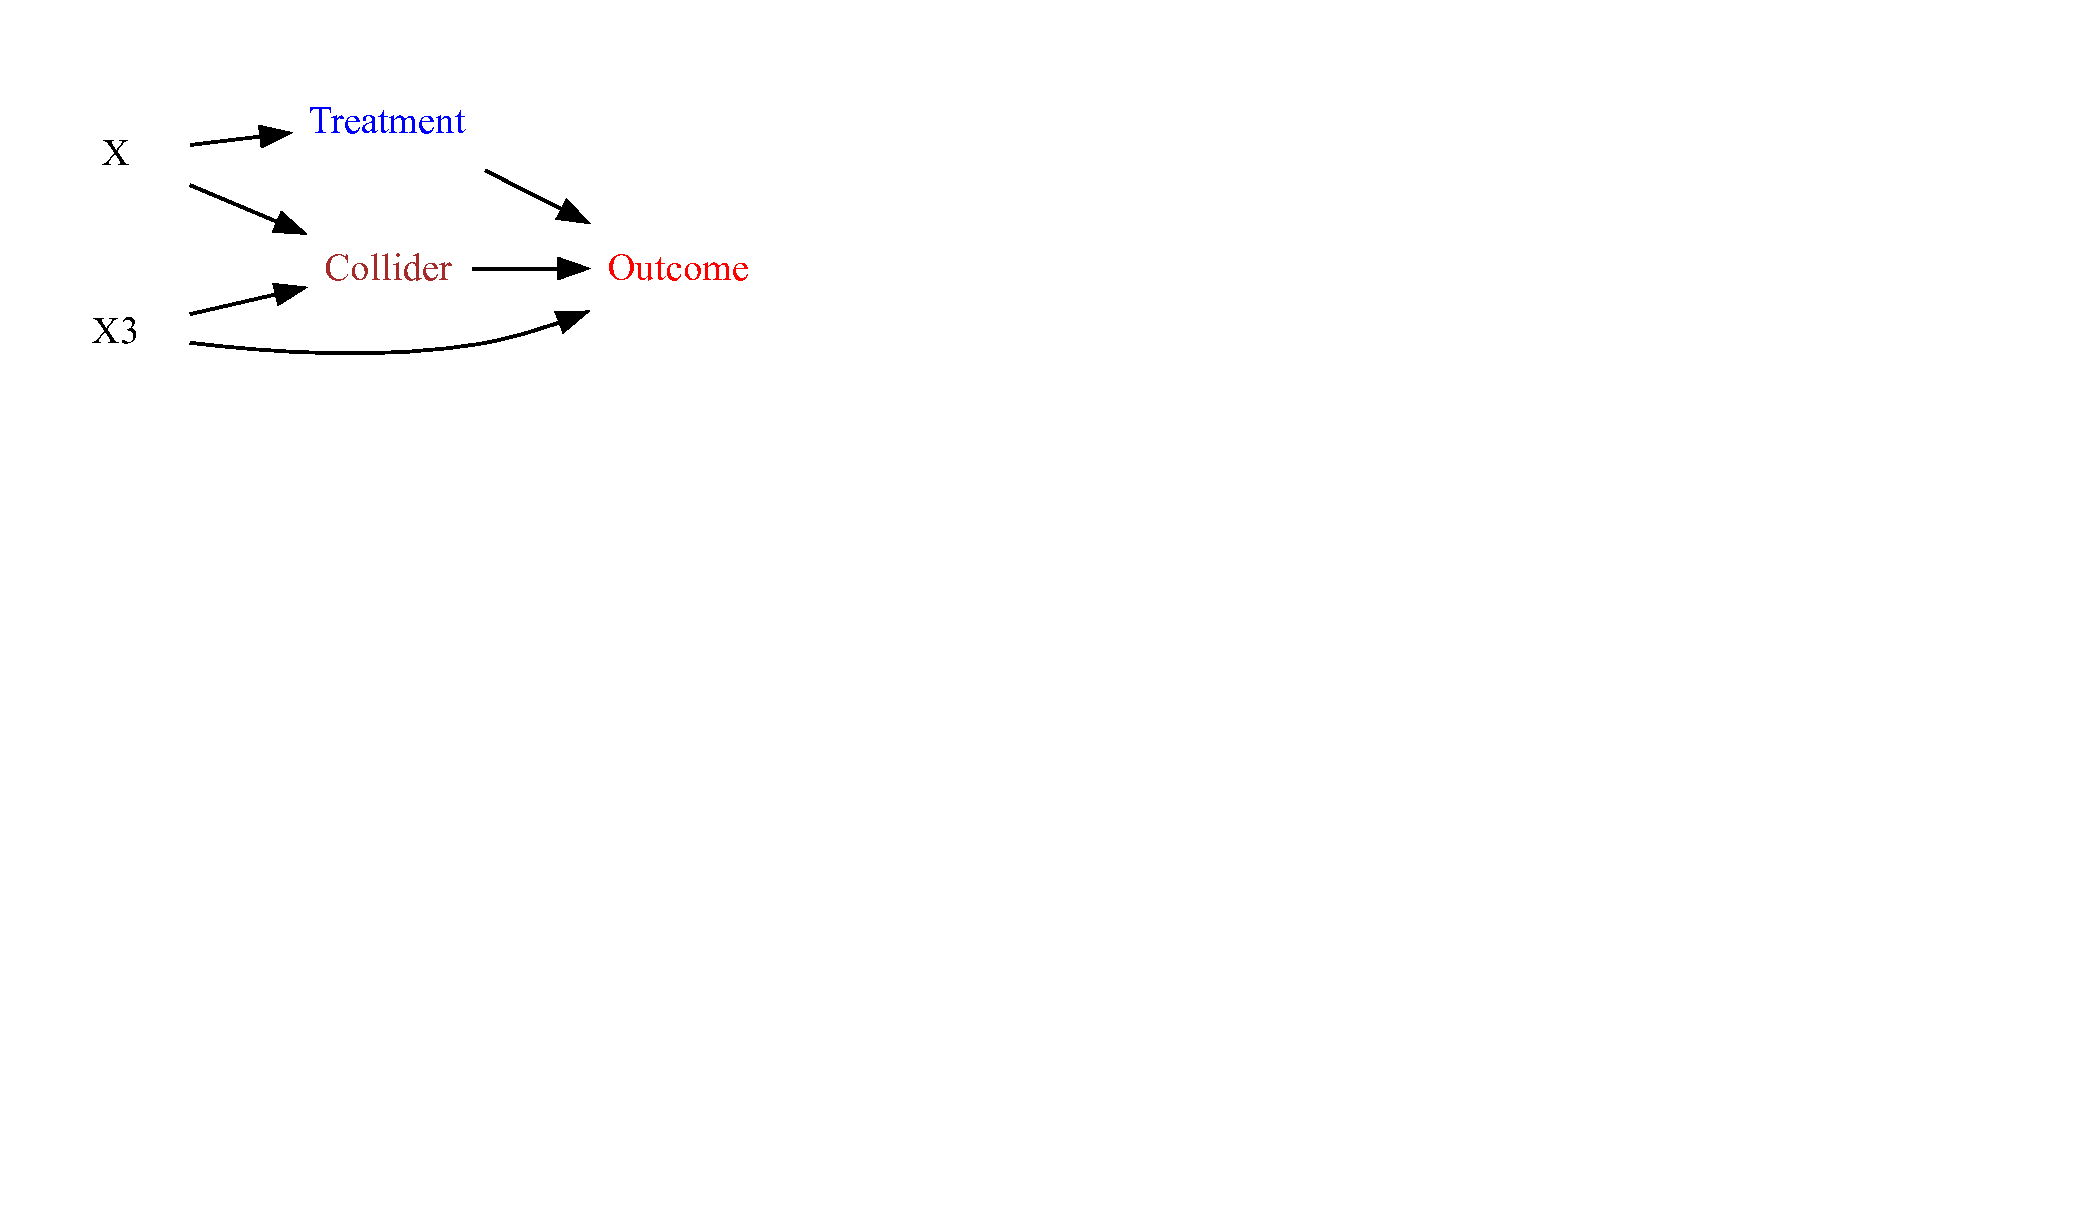
\includegraphics[width=2.7\linewidth]{figure/Dag5-1} 

\end{knitrout}
\end{frame}

\begin{frame}
\frametitle{3. Colliders}
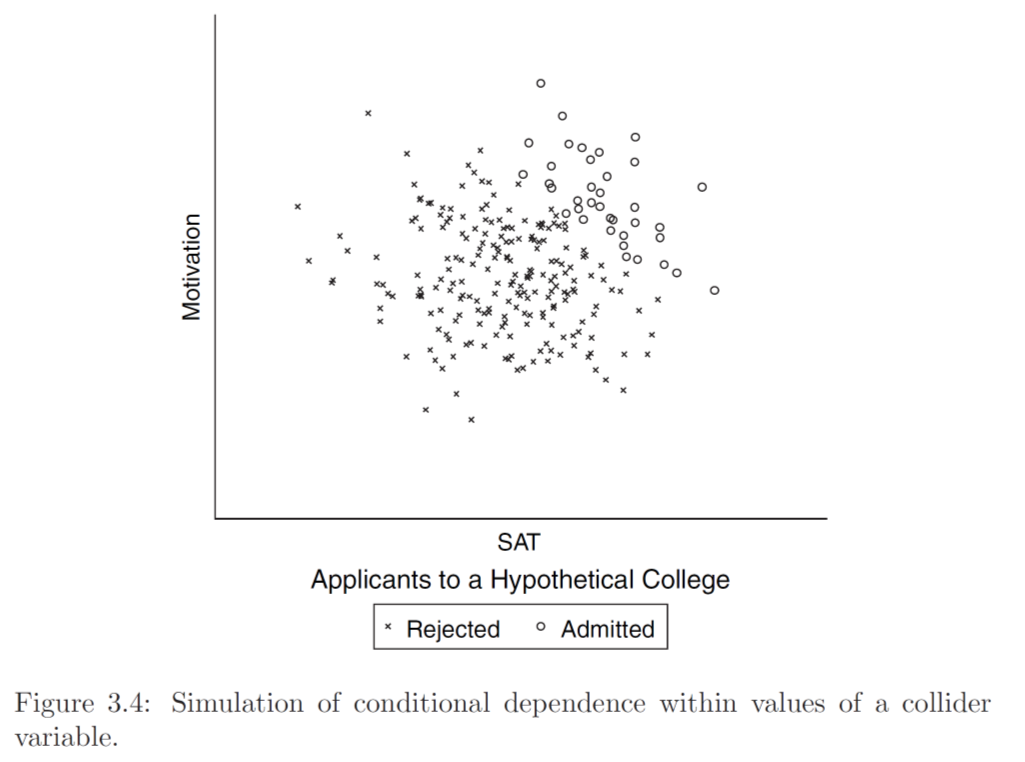
\includegraphics[width=0.9\textwidth]{Collider.png}
\end{frame}

\begin{frame}
\frametitle{3. Colliders}
\begin{knitrout}
\definecolor{shadecolor}{rgb}{0.969, 0.969, 0.969}\color{fgcolor}
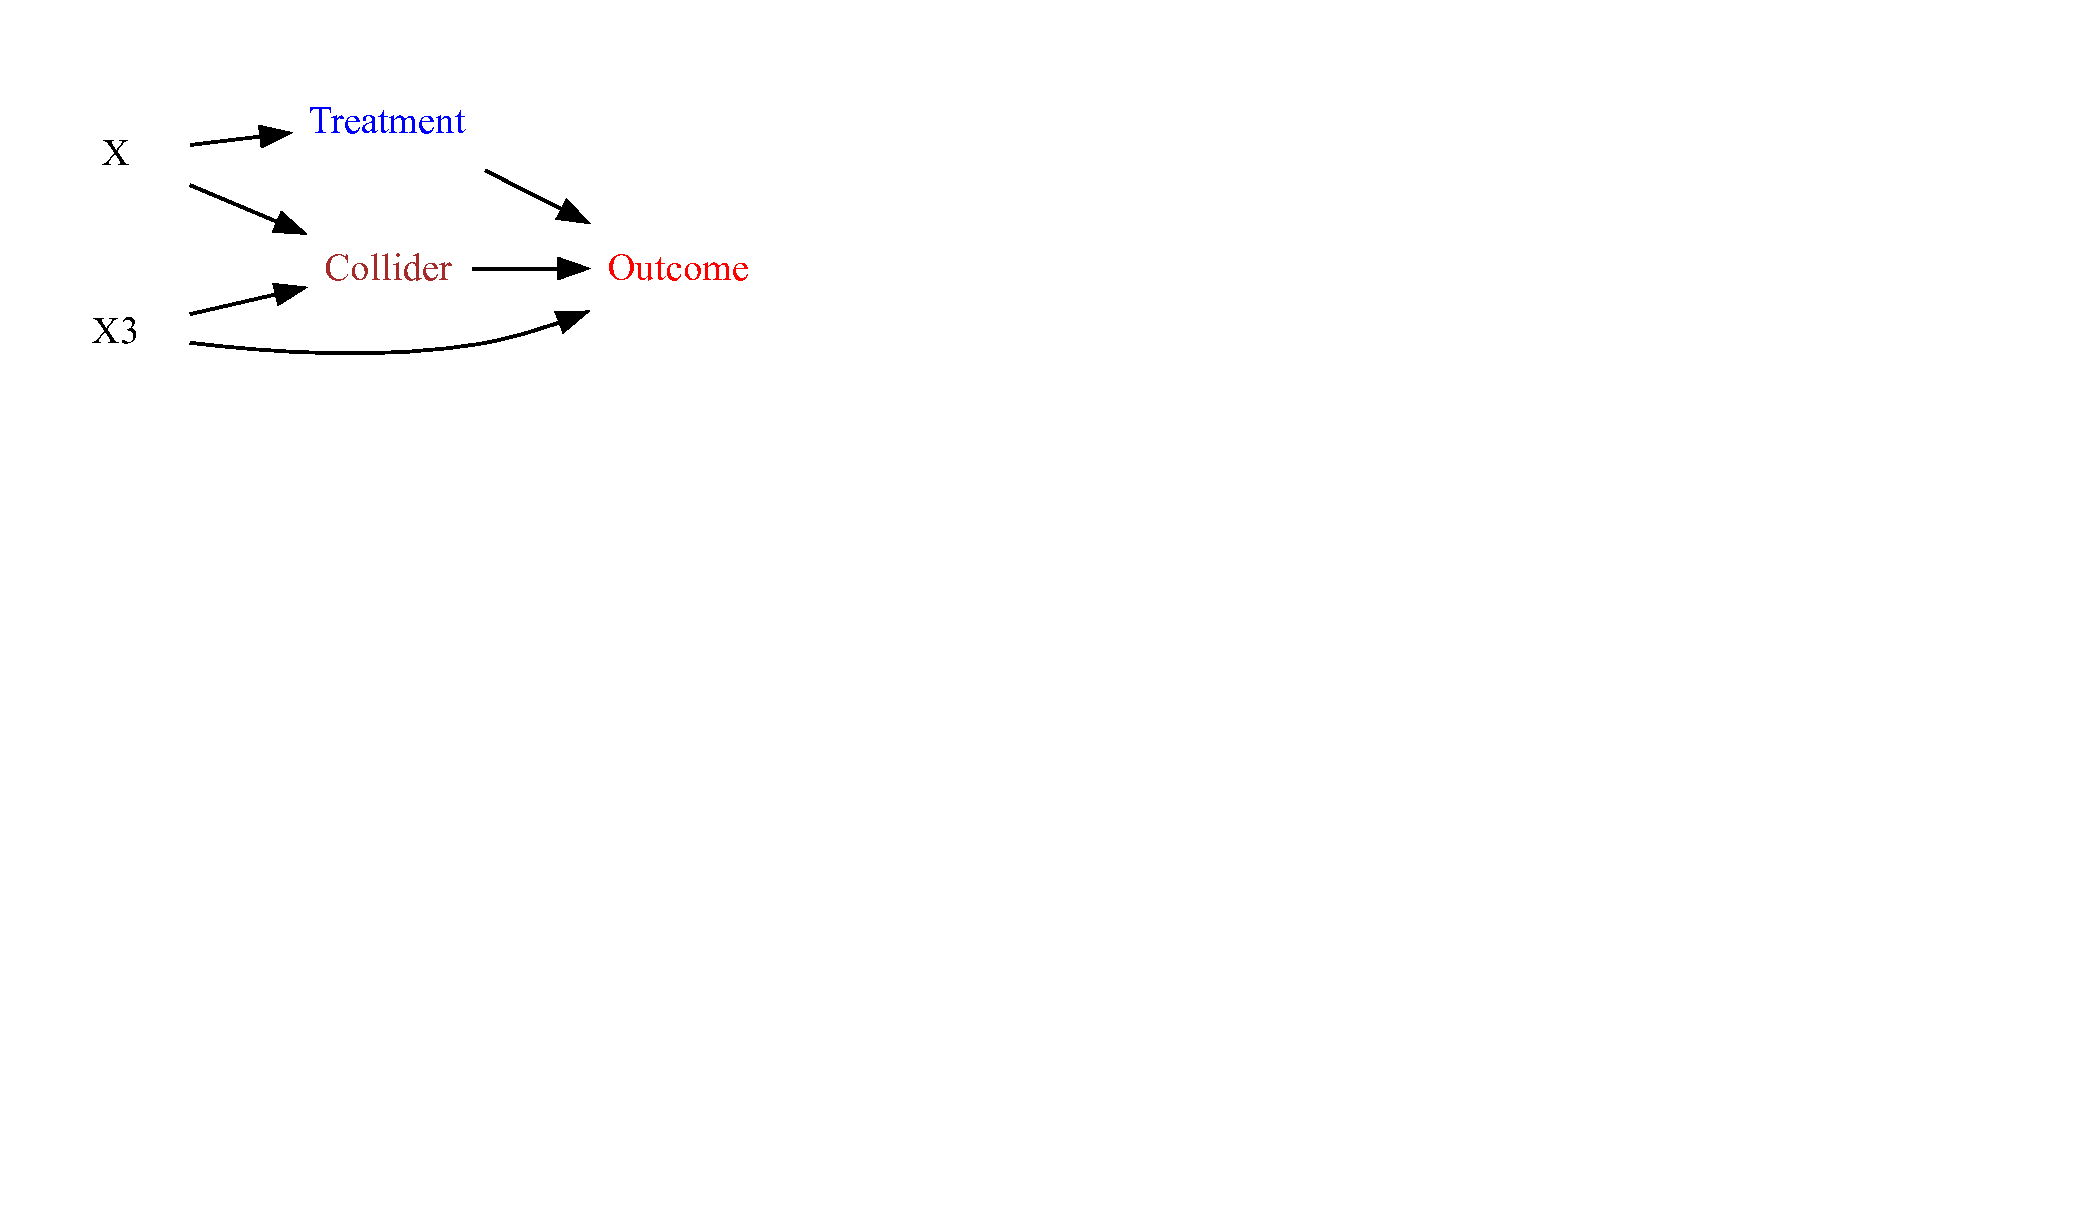
\includegraphics[width=2.7\linewidth]{figure/Dag5b-1} 

\end{knitrout}
\end{frame}

\begin{frame}
\frametitle{Example adapted from Morgan and Winship, p.72}
\begin{enumerate}
\footnotesize
\item List all of the \textbf{back-door paths} from $D$ to $Y$
\pause
\item Identify any \textbf{post-treatment} variables: Do NOT include as controls
\pause
\item Identify any back-door paths with \textbf{collider} variables: Mark these as already blocked
\pause
\item Find a minimum set of variables that blocks all remaining back-door paths
\pause
\item Double-check your minimum set of control variables does not contain any post-treatment or collider variables
\end{enumerate}
\normalsize
\begin{knitrout}
\definecolor{shadecolor}{rgb}{0.969, 0.969, 0.969}\color{fgcolor}
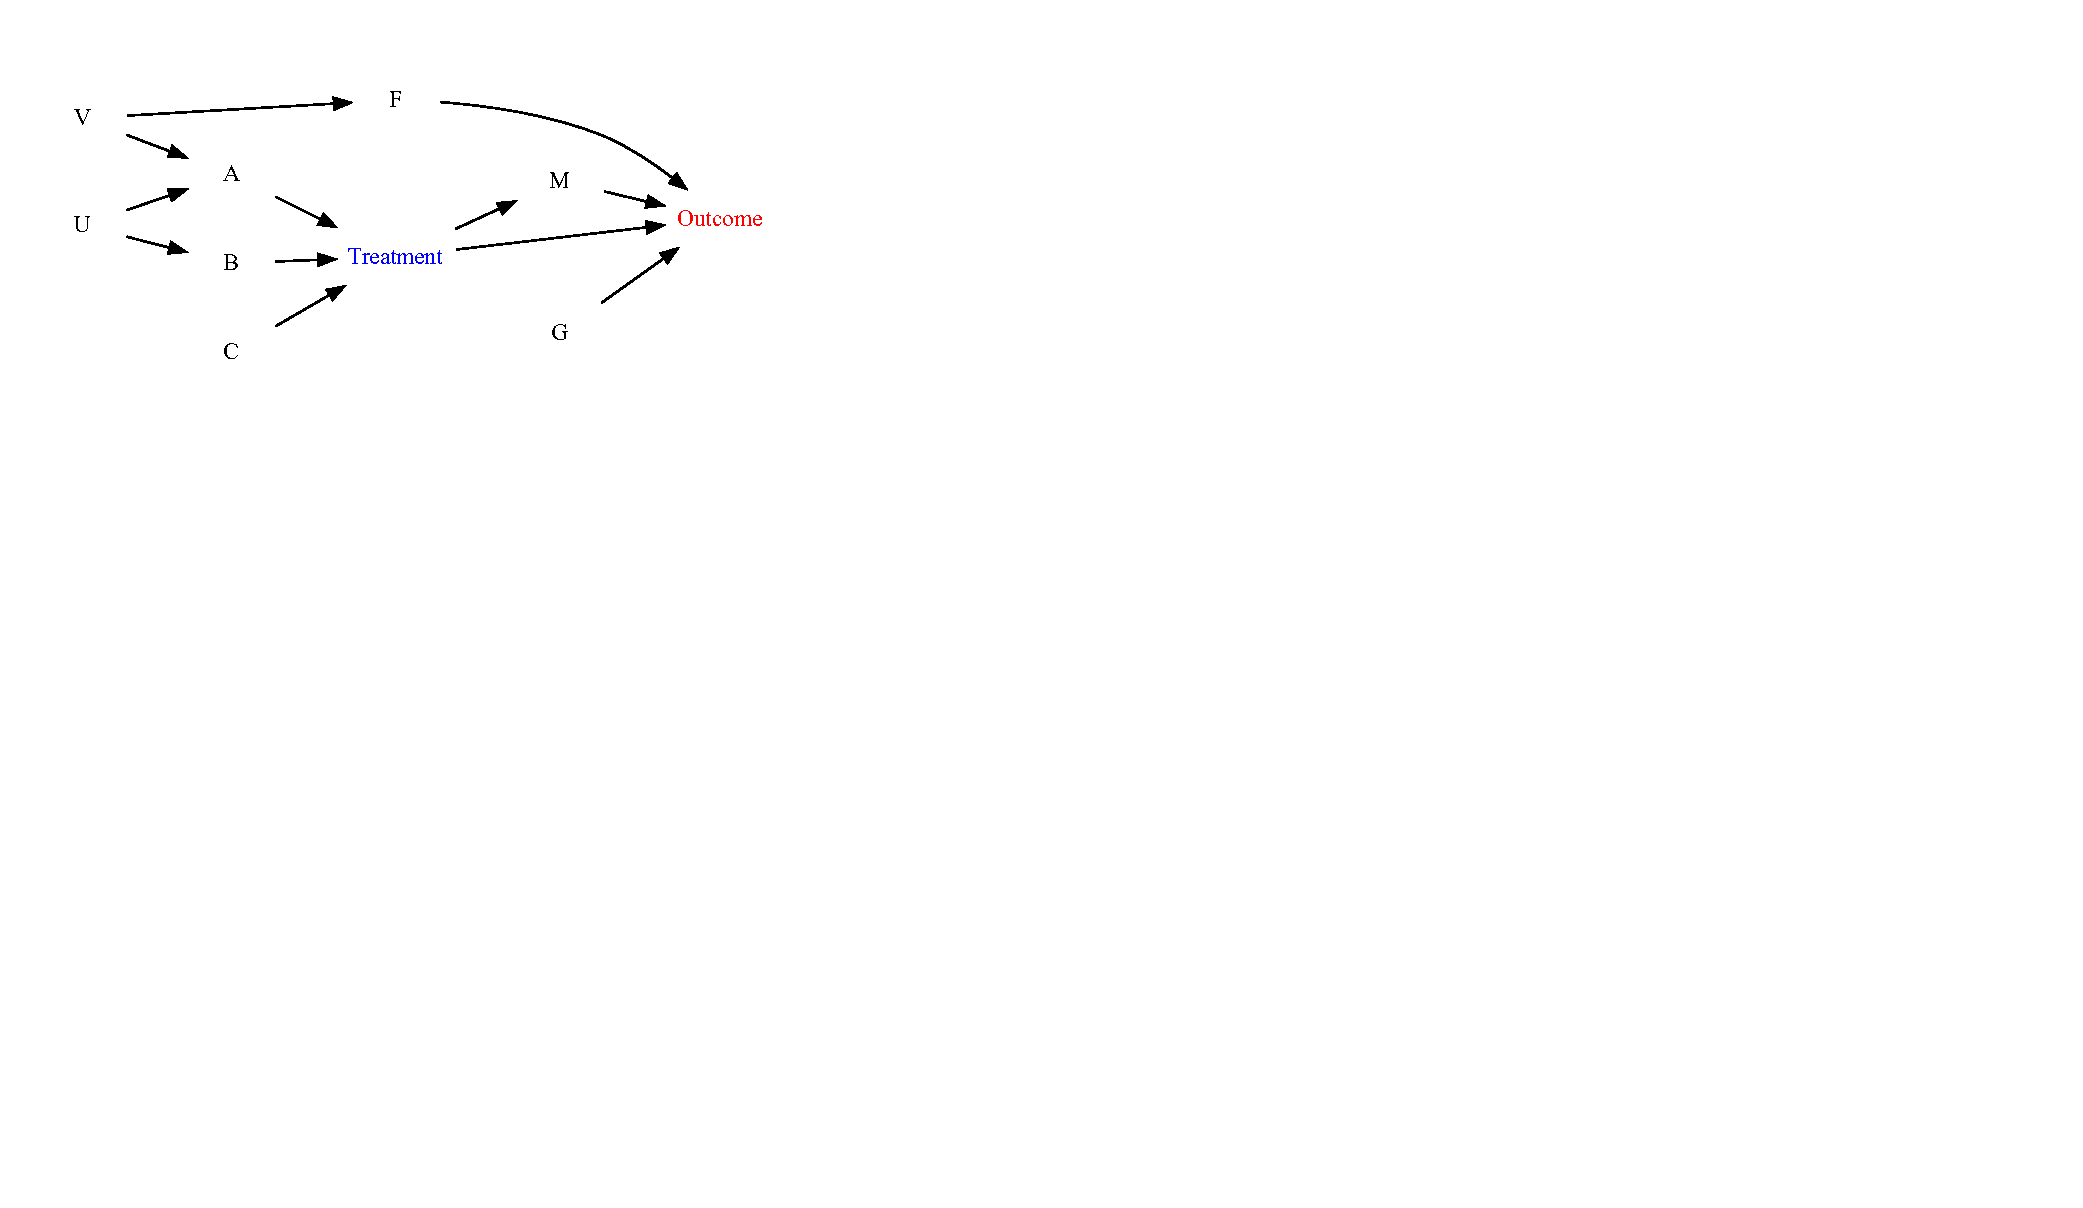
\includegraphics[width=2.4\linewidth]{figure/Dag5_eg-1} 

\end{knitrout}
\end{frame}

\begin{frame}
\frametitle{Causal Diagrams (DAGs)}
\begin{itemize}
\item Three Rules to achieve Conditional Independence:
\begin{enumerate}
\item Include as controls enough variables to \textbf{block all back-door paths} from treatment to the outcome
\pause
\begin{itemize}
\item In practice, variables which theory and past studies identify as potential confounders
\end{itemize}
\pause
\item Exclude any variables that are \textbf{post-treatment}
\pause
\begin{itemize}
\item In practice, know when your variables were measured
\end{itemize}
\pause
\item Exclude any variables that are \textbf{colliders}
\pause
\begin{itemize}
\item In practice, don't include unnecessary controls
\end{itemize}
\end{enumerate}
\end{itemize}
\end{frame}


\end{document}
